% ============================================================================
% Deep Equilibrium Nets (DEQNs)
% Summer School on AI for Economics and Finance
% University of Torino, August 24, 2026
% Duration: 75--90 minutes
% ============================================================================

\documentclass[aspectratio=169,11pt]{beamer}

% ---------- Theme and colors ----------
\usecolortheme{dove}
\setbeamertemplate{navigation symbols}{}
\setbeamertemplate{footline}{%
  \hfill\usebeamerfont{page number in head/foot}%
  \usebeamercolor[fg]{normal text}%
  \insertframenumber\,/\,\inserttotalframenumber\kern1em\vskip4pt}
\setbeamerfont{frametitle}{size=\huge}

% ---------- Packages ----------
\usepackage[utf8]{inputenc}
\usepackage[T1]{fontenc}
\usepackage{amsmath,amssymb,amsfonts}
\usepackage{bm}
\usepackage{graphicx}
\usepackage{tikz}
\usetikzlibrary{shapes,arrows.meta,positioning,calc,fit,backgrounds,patterns,decorations.pathreplacing}
\usepackage{pgfplots}
\pgfplotsset{compat=1.18}
% --- readable-from-the-back defaults for every plot ---
\pgfplotsset{every axis/.append style={
    tick label style={font=\footnotesize},
    label style={font=\small},
    title style={font=\small},
    legend style={font=\footnotesize}}}
\usepgfplotslibrary{fillbetween}
\usepackage{booktabs}
\usepackage{hyperref}
\usepackage{multicol}
\usepackage{xcolor}
\usepackage{algorithmic}

% ---------- Tighter display math, applied uniformly at every font size ------
% (a global typographic setting, so that no frame needs a local \vspace hack)
\makeatletter
\g@addto@macro\normalsize{%
  \setlength\abovedisplayskip{5pt plus 2pt minus 2pt}%
  \setlength\belowdisplayskip{5pt plus 2pt minus 2pt}%
  \setlength\abovedisplayshortskip{2pt plus 1pt}%
  \setlength\belowdisplayshortskip{3pt plus 1pt}}
\g@addto@macro\small{%
  \setlength\abovedisplayskip{4pt plus 2pt minus 2pt}%
  \setlength\belowdisplayskip{4pt plus 2pt minus 2pt}%
  \setlength\abovedisplayshortskip{2pt plus 1pt}%
  \setlength\belowdisplayshortskip{2pt plus 1pt}}
\g@addto@macro\footnotesize{%
  \setlength\abovedisplayskip{3pt plus 2pt minus 2pt}%
  \setlength\belowdisplayskip{3pt plus 2pt minus 2pt}%
  \setlength\abovedisplayshortskip{1pt plus 1pt}%
  \setlength\belowdisplayshortskip{2pt plus 1pt}}
\makeatother

% ---------- Custom colors ----------
\definecolor{uzhblue}{rgb}{0,0,0.5}
\definecolor{uzhgreylight}{RGB}{236,238,241}
\definecolor{uzhgreydark}{RGB}{81,86,94}
\definecolor{harvardcrimson}{RGB}{153,0,0}
\definecolor{unil@blue}{RGB}{0,140,204}
\definecolor{unil@black}{RGB}{35,31,32}
\definecolor{darkgreen}{RGB}{0,100,0}
\definecolor{darkred}{RGB}{139,0,0}
\definecolor{softblue}{RGB}{70,130,180}
\definecolor{softorange}{RGB}{230,159,0}
\definecolor{softgreen}{RGB}{0,158,115}

% ---------- Set beamer colors ----------
\setbeamercolor{frametitle}{bg=uzhgreylight, fg=uzhblue}
\setbeamercolor{title}{fg=uzhblue}
\setbeamercolor{structure}{fg=uzhblue}
\setbeamercolor{block title}{bg=unil@blue, fg=white}
\setbeamercolor{block body}{bg=uzhgreylight}
\setbeamercolor{block title alerted}{bg=darkred,fg=white}
\setbeamercolor{block body alerted}{bg=red!5}
\setbeamercolor{block title example}{bg=darkgreen,fg=white}
\setbeamercolor{block body example}{bg=green!5}
\setbeamercolor{item}{fg=unil@black}
\setbeamercolor{normal text}{fg=unil@black}

% ---------- Emphasis and hyperlinks ----------
\newcommand{\emphc}[1]{\textcolor{harvardcrimson}{#1}}
\hypersetup{colorlinks,linkcolor=harvardcrimson,urlcolor=harvardcrimson}

% ---------- Math commands ----------
% One symbol, one meaning. See the notation frame in Part II.
\newcommand{\x}{\bm{x}}
\newcommand{\bb}{\bm{b}}
\newcommand{\W}{\bm{W}}
\renewcommand{\a}{\bm{a}}
\newcommand{\R}{\mathbb{R}}
\newcommand{\E}[1]{\mathbb{E}\!\left[#1\right]}
\newcommand{\Et}[1]{\mathbb{E}_t\!\left[#1\right]}
\newcommand{\param}{\theta}          % network parameters (one typeface)
\newcommand{\state}{\bm{x}}          % state vector (same glyph as \x)
\newcommand{\resid}{\mathcal{R}}     % equilibrium residual (one name)
\newcommand{\net}{\mathcal{N}_{\param}} % the network
\newcommand{\cov}{\mu_{\mathrm{cov}}}
\newcommand{\Lag}{\Lambda}           % Lagrangian (never the loss)

% ---------- Title ----------
\title[DEQNs -- Torino 2026]%
{Summer School on AI for Economics and Finance}
\subtitle{Deep Equilibrium Nets: from Brock--Mirman to loss balancing and architecture search}
\author{Simon Scheidegger}
\institute[HEC Lausanne]{HEC, University of Lausanne\\[4pt]
{\footnotesize Based on Azinovic, Gaegauf \& Scheidegger (2022), \emph{International Economic Review} 63(4), 1471--1525}}
\date{University of Torino\\August 24, 2026}

\begin{document}

% ============================================================================
% PART 0: TITLE & OUTLINE
% ============================================================================

% --- Slide 1: Title ---
{\setbeamercolor{background canvas}{bg=uzhgreylight}
\begin{frame}
\titlepage
\end{frame}
}

% --- Slide 2: Day 1 at a glance (same frame as lecture 1) ---
\begin{frame}{Day 1 at a Glance}
\begin{center}
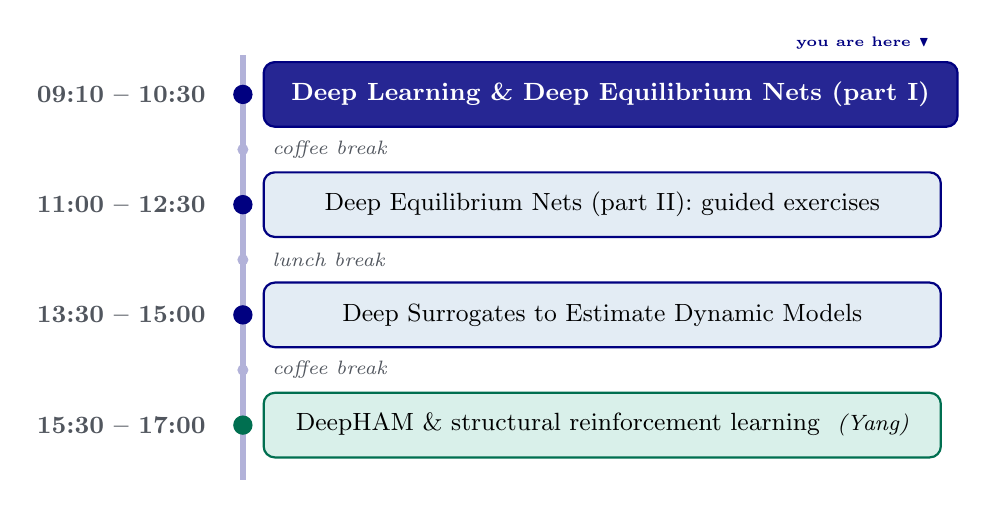
\begin{tikzpicture}[
    session/.style={rectangle, rounded corners=4pt, draw=uzhblue, thick, fill=softblue!15,
                    minimum width=8.6cm, minimum height=0.82cm, align=left, font=\small,
                    inner xsep=10pt, anchor=west},
    now/.style={session, fill=uzhblue!85, draw=uzhblue, text=white, font=\small\bfseries},
    guest/.style={session, fill=softgreen!15, draw=softgreen!70!black},
    pause/.style={font=\scriptsize\itshape, text=uzhgreydark, anchor=west},
    time/.style={font=\small\bfseries, text=uzhgreydark, anchor=east}
]
    \draw[uzhblue!30, line width=2pt] (0,0.5) -- (0,-4.9);

    \node[time] at (-0.35, 0) {09:10 -- 10:30};
    \node[now]  at (0.25, 0) {Deep Learning \& Deep Equilibrium Nets (part I)};
    \fill[uzhblue] (0,0) circle (3.5pt);
    \node[font=\tiny\bfseries, text=uzhblue, anchor=south east] at (8.85,0.45) {you are here $\blacktriangledown$};

    \node[pause] at (0.25,-0.7) {coffee break};
    \fill[uzhblue!30] (0,-0.7) circle (2pt);

    \node[time] at (-0.35,-1.4) {11:00 -- 12:30};
    \node[session] at (0.25,-1.4) {Deep Equilibrium Nets (part II): guided exercises};
    \fill[uzhblue] (0,-1.4) circle (3.5pt);

    \node[pause] at (0.25,-2.1) {lunch break};
    \fill[uzhblue!30] (0,-2.1) circle (2pt);

    \node[time] at (-0.35,-2.8) {13:30 -- 15:00};
    \node[session] at (0.25,-2.8) {Deep Surrogates to Estimate Dynamic Models};
    \fill[uzhblue] (0,-2.8) circle (3.5pt);

    \node[pause] at (0.25,-3.5) {coffee break};
    \fill[uzhblue!30] (0,-3.5) circle (2pt);

    \node[time] at (-0.35,-4.2) {15:30 -- 17:00};
    \node[guest] at (0.25,-4.2) {DeepHAM \& structural reinforcement learning~~{\footnotesize\itshape (Yang)}};
    \fill[softgreen!70!black] (0,-4.2) circle (3.5pt);
\end{tikzpicture}
\end{center}

\vspace{0.1cm}
\begin{center}
{\footnotesize \textbf{Materials:}~\href{https://github.com/sischei/summer-school-AI-for-economics-and-finance-2026}{github.com/sischei/summer-school-AI-\ldots-2026}~~$\cdot$~~\textbf{Cloud:}~\href{https://nuvolos.cloud}{nuvolos.cloud}}
\end{center}
\end{frame}

% --- Slide 3: Roadmap ---
\begin{frame}{Roadmap of This Lecture (75--90 min)}
\begin{columns}[T]
\column{0.48\textwidth}
\textbf{I.\ Motivation}~~\mbox{\small (12 min)}
\begin{itemize}\setlength\itemsep{1pt}
    \item Heterogeneity, high dimensions, kinks, irregular ergodic sets
\end{itemize}

\vspace{0.5em}
\textbf{II.\ From neural networks to DEQNs}~~\mbox{\small (13 min)}
\begin{itemize}\setlength\itemsep{1pt}
    \item Self-supervised loss, the training algorithm, where DEQNs sit
\end{itemize}

\vspace{0.5em}
\textbf{III.\ Brock--Mirman benchmark}~~\mbox{\small (25 min)}
\begin{itemize}\setlength\itemsep{1pt}
    \item Euler equation, hard constraints, residual and loss
    \item Quadrature, diagnostics, validation, loss kernels
\end{itemize}

\column{0.48\textwidth}
\textbf{IV.\ Loss balancing}~~\mbox{\small (15 min)}
\begin{itemize}\setlength\itemsep{1pt}
    \item Pathology (a): components at different scales
\end{itemize}

\vspace{0.5em}
\textbf{V.\ Architecture search}~~\mbox{\small (13 min)}
\begin{itemize}\setlength\itemsep{1pt}
    \item Pathology (b): random search and Hyperband
\end{itemize}

\vspace{0.5em}
\textbf{VI.\ Further pathologies, HPC, wrap-up}~~\mbox{\small (12 min)}
\begin{itemize}\setlength\itemsep{1pt}
    \item Pathologies (c) to (e), data parallelism, hands-on preview
\end{itemize}
\end{columns}
\end{frame}

% --- Slide 4: Learning objectives ---
\begin{frame}{Learning Objectives}
\textbf{By the end of this lecture you should be able to:}
\begin{itemize}\itemsep3pt
  \item Formulate dynamic stochastic economic models as equilibrium systems and identify the computational challenges in high dimensions
  \item Replace grid-based collocation with \emphc{self-supervised} neural-network training that uses equilibrium errors as the loss
  \item Build and train Deep Equilibrium Nets (DEQNs), and validate one against the Brock--Mirman closed form
  \item Diagnose and cure the two most common failure modes in practice: \emphc{loss-scale imbalance} and \emphc{poor architecture choice}
  \item Recognize the three residual-only pathologies that remain: lazy learning, learning from scratch, and self-confirming coverage
  \item Know when to reach for adaptive loss balancing (ReLoBRaLo), automated architecture search, and data parallelism
\end{itemize}
\end{frame}

% ============================================================================
% PART I: MOTIVATION
% ============================================================================

\section{Motivation}

\begin{frame}{}
\begin{center}
{\Huge \textcolor{uzhblue}{Part I}}\\[0.8em]
{\LARGE Motivation}
\end{center}
\end{frame}

% --- Heterogeneity ---
\begin{frame}{Heterogeneity Matters}
\begin{columns}[T]
\column{0.50\textwidth}
\textbf{The questions:} inequality over the life cycle, idiosyncratic versus aggregate risk, distributional effects of policy.

\vspace{0.4em}
\textbf{The punchline:} \emphc{hand-to-mouth} households have a quarterly MPC of roughly $0.3$ to $0.5$, against about $0.05$ for unconstrained ones. A representative agent averages these out and misses the policy response.

\vspace{0.3em}
{\footnotesize Kaplan, Moll \& Violante 2018; Bilbiie 2008; Krueger, Mitman \& Perri 2016}

\vspace{0.4em}
$\Rightarrow$ Heterogeneity is one of several forces that \emphc{blow up} the state dimension $d_x$.

\column{0.48\textwidth}
\begin{center}
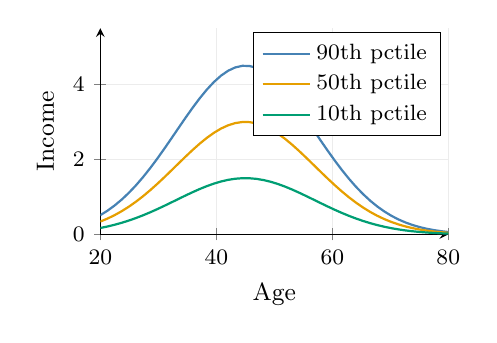
\begin{tikzpicture}
\begin{axis}[
    width=6.0cm, height=4.2cm,
    xlabel={Age}, ylabel={Income},
    xmin=20, xmax=80, ymin=0, ymax=5.5,
    grid=major, grid style={gray!15},
    legend style={at={(0.98,0.98)}, anchor=north east},
    axis lines=left,
]
    \addplot[thick, softblue, domain=20:80, samples=50]
        {4.5*exp(-0.5*((x-45)/12)^2)};
    \addlegendentry{90th pctile}
    \addplot[thick, softorange, domain=20:80, samples=50]
        {3.0*exp(-0.5*((x-45)/12)^2)};
    \addlegendentry{50th pctile}
    \addplot[thick, softgreen, domain=20:80, samples=50]
        {1.5*exp(-0.5*((x-45)/12)^2)};
    \addlegendentry{10th pctile}
\end{axis}
\end{tikzpicture}\\
{\footnotesize Stylized income-by-age profiles}
\end{center}
\end{columns}
\end{frame}

% --- DSGE models ---
\begin{frame}{Dynamic Stochastic General Equilibrium Models}
\textbf{Generic formulation:} find policy functions $p(\cdot)$ such that
\[
\Et{\resid\bigl(\state_t,\,\state_{t+1},\,p(\state_t),\,p(\state_{t+1})\bigr)} = 0
\]
with transition law $\state_{t+1} = h\bigl(\state_t,\,p(\state_t),\,\bm\varepsilon_{t+1}\bigr)$, where $\resid$ collects the equilibrium conditions.

\vspace{0.4em}
\textbf{Four computational challenges} (Azinovic, Gaegauf \& Scheidegger, 2022):
\begin{enumerate}
    \setlength{\itemsep}{1pt}
    \item \emphc{Stochasticity}: nontrivial expectations over $\bm\varepsilon_{t+1}$ and over the ergodic distribution
    \item \emphc{High-dimensional} state space: heterogeneity, many assets, and many shocks all push $d_x$ up
    \item \emphc{Strong nonlinearities and kinks} from occasionally binding constraints and regime switches
    \item \emphc{Irregular geometry} of the ergodic set: recurrent states are not a hypercube
\end{enumerate}

\vspace{0.2em}
{\footnotesize No classical method addresses all four jointly: sparse grids cover (1)--(3) but become impractical past $d_x \sim 20$; Gaussian processes cover (1), (2) and (4) but cost $\mathcal{O}(n^3)$ to train.}
\end{frame}

% --- What is high-dimensional ---
\begin{frame}{What Is High-Dimensional?}
\begin{center}
\begin{tabular}{rrl}
\toprule
\textbf{Dimensions $d_x$} & \textbf{Grid points $n_g^{d_x}$} & \textbf{Runtime} \\
\midrule
1 & $10$ & 10 seconds \\
2 & $100$ & 2 minutes \\
5 & $10^5$ & 1 day \\
10 & $10^{10}$ & 317 years \\
20 & $10^{20}$ & $\sim 3$ trillion years \\
\bottomrule
\end{tabular}
\end{center}

\vspace{0.5em}
{\small Assumes $n_g = 10$ grid points per dimension and 1 second per evaluation. This is the curse of dimensionality of lecture 1, now with an economic state on the axis.}

\vspace{0.5em}
\textbf{Three remedies:}
\begin{enumerate}
    \item \emphc{Sparse grids} (Brumm \& Scheidegger, 2017)
    \item \emphc{Random grids} (Rust, 1997), for the restricted class of discrete decision processes
    \item \emphc{Neural networks} (this lecture)
\end{enumerate}
\end{frame}

% --- Nonlinearities and kinks ---
\begin{frame}{Nonlinearities and Kinks}
\begin{columns}[T]
\column{0.52\textwidth}
\textbf{Where do kinks come from?}
\begin{itemize}
    \setlength{\itemsep}{1pt}
    \item \emphc{Borrowing constraints}: $a_{t+1}\ge \underline{a}$
    \item \emphc{Zero lower bound}: $i_t \ge 0$
    \item \emphc{Short-sale and participation}: corner solutions
    \item \emphc{Default, regime switches, indivisibilities}
\end{itemize}

\vspace{0.4em}
Occasionally binding constraints $\Rightarrow$ policy functions are \emphc{non-smooth} at the boundary of the binding region.

\vspace{0.4em}
{\footnotesize Polynomial and spectral methods lose accuracy; sparse grids can resolve kinks but only for $d_x\lesssim 20$. Neural networks handle kinks natively via ReLU-type activations.}

\column{0.48\textwidth}
\begin{center}
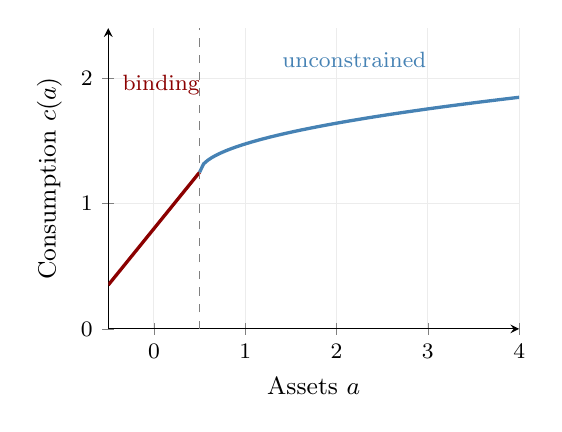
\begin{tikzpicture}
\begin{axis}[
    width=6.8cm, height=5.4cm,
    xlabel={Assets $a$}, ylabel={Consumption $c(a)$},
    xmin=-0.5, xmax=4, ymin=0, ymax=2.4,
    grid=major, grid style={gray!15},
    axis lines=left,
    samples=80,
]
    \addplot[very thick, darkred, domain=-0.5:0.5] {0.35 + 0.90*(x+0.5)};
    \addplot[very thick, softblue, domain=0.5:4] {1.25 + 0.32*sqrt(x-0.5)};
    \draw[dashed, gray] (axis cs:0.5,0) -- (axis cs:0.5,2.4);
    \node[font=\footnotesize, anchor=north] at (axis cs:0.5,0) {$a=\underline{a}$};
    \node[font=\footnotesize, darkred, anchor=west] at (axis cs:-0.45,1.95) {binding};
    \node[font=\footnotesize, softblue, anchor=west] at (axis cs:1.3,2.15) {unconstrained};
\end{axis}
\end{tikzpicture}\\
{\footnotesize Kinked consumption policy at the borrowing limit}
\end{center}
\end{columns}
\end{frame}

% --- Ergodic set ---
\begin{frame}{The Ergodic Set Is Not a Hypercube}
\textbf{Grid-based} methods tile the full hypercube $\state \in [\state_{\min}, \state_{\max}]^{d_x}$. \textbf{But} simulated states drawn from the model's law of motion fill only a \emphc{thin, irregular} subset, the \emphc{ergodic set} of states the economy actually visits, often $\ll 1\%$ of the hypercube {\footnotesize (Judd, Maliar \& Maliar, 2011)}.

\vspace{0.3em}
\begin{center}
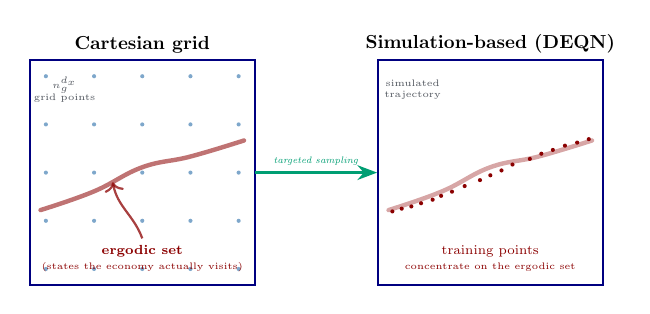
\begin{tikzpicture}[scale=0.68, transform shape,
    dotblue/.style={circle, fill=softblue!70, inner sep=0pt, minimum size=2.2pt},
    dotred/.style={circle, fill=darkred,      inner sep=0pt, minimum size=2.2pt},
    cube/.style={rectangle, draw=uzhblue, thick, minimum width=4.2cm, minimum height=4.2cm}]
    \node[cube, label={above:\textbf{Cartesian grid}}] (g) at (0,0) {};
    \foreach \i in {-1.8,-0.9,0,0.9,1.8} {
        \foreach \j in {-1.8,-0.9,0,0.9,1.8} {
            \node[dotblue] at (\i,\j) {};
        }
    }
    \draw[darkred, ultra thick, opacity=0.55, line cap=round]
        plot[smooth, tension=0.7] coordinates {(-1.9,-0.7) (-0.9,-0.35) (0,0.1) (0.9,0.3) (1.9,0.6)};
    \node[font=\scriptsize, text=darkred, align=center] (ergL) at (0,-1.6)
        {\textbf{ergodic set}\\{\tiny (states the economy actually visits)}};
    \draw[->, darkred, thick, opacity=0.75]
        (ergL.north) to[out=110,in=-80,looseness=1.0] (-0.55,-0.18);
    \node[font=\tiny, text=uzhgreydark, align=center] at (-1.45,1.55) {$n_g^{d_x}$\\grid points};

    \node[cube, label={above:\textbf{Simulation-based (DEQN)}}] (s) at (6.5,0) {};
    \begin{scope}[xshift=6.5cm]
        \draw[darkred, ultra thick, opacity=0.35, line cap=round]
            plot[smooth, tension=0.7] coordinates {(-1.9,-0.7) (-0.9,-0.35) (0,0.1) (0.9,0.3) (1.9,0.6)};
        \foreach \t in {-1.85,-1.65,-1.5,-1.3,-1.1,-0.9,-0.7,-0.45,-0.2,0,0.2,0.45,0.7,0.95,1.15,1.4,1.6,1.85}{
            \pgfmathsetmacro{\yy}{-0.7 + 1.3*(\t + 1.9)/3.8 + 0.08*sin(deg(\t*1.4))}
            \pgfmathsetmacro{\xx}{\t + 0.04*rand}
            \node[dotred] at (\xx,\yy) {};
        }
        \node[font=\tiny, text=uzhgreydark, align=center] at (-1.45,1.55)
            {simulated\\trajectory};
        \node[font=\scriptsize, text=darkred, align=center] at (0,-1.6)
            {training points\\{\tiny concentrate on the ergodic set}};
    \end{scope}

    \draw[-{Stealth[length=2.5mm]}, thick, softgreen]
        (g.east) -- node[above, font=\tiny, text=softgreen]{\textit{targeted sampling}} (s.west);
\end{tikzpicture}
\end{center}

\begin{center}
{\footnotesize A full Cartesian grid \emphc{wastes} most of its work in regions the economy never visits, which motivates \emphc{simulation-based, grid-free} methods.}
\end{center}
\end{frame}

% --- Wishlist and answer (merged) ---
\begin{frame}{What We Need, and What DEQNs Deliver}
\begin{columns}[T]
\column{0.46\textwidth}
\textbf{The wishlist.} A numerical method that is
\begin{enumerate}
    \setlength{\itemsep}{2pt}
    \item \textbf{global}, not a local perturbation;
    \item content with a small residual error;
    \item \textbf{grid-free}, avoiding growth like $n_g^{d_x}$;
    \item comfortable with kinks and irregular ergodic sets;
    \item \textbf{parallel-friendly}.
\end{enumerate}

\column{0.50\textwidth}
\begin{block}{Three ingredients (Azinovic, Gaegauf \& Scheidegger, 2022)}
\begin{enumerate}\itemsep2pt
    \item \textbf{Equilibrium error as the loss:} use $\resid(\cdot) = 0$ directly, with \emphc{no labeled data}
    \item \textbf{Stochastic gradient descent} on the parameters $\param$
    \item \textbf{Simulated paths:} draw training points from the model's own \emphc{ergodic distribution}
\end{enumerate}
\end{block}
\end{columns}

\vspace{0.4em}
\begin{center}
{\footnotesize $\Rightarrow$ This turns \emphc{solving} an economic model into \emphc{training} a neural network, while \emphc{mitigating} rather than eliminating high-dimensional costs: expectation accuracy, sampling quality, and optimization all still matter.}
\end{center}
\end{frame}

% ============================================================================
% PART II: FROM NEURAL NETWORKS TO DEQNs
% ============================================================================

\section{From Neural Networks to DEQNs}

\begin{frame}{}
\begin{center}
{\Huge \textcolor{uzhblue}{Part II}}\\[0.8em]
{\LARGE From Neural Networks to DEQNs}
\end{center}
\end{frame}

% --- What we carry over from lecture 1 (merged recap) ---
\begin{frame}{What We Carry Over From Lecture 1}
A deep network composes affine maps with activations, with $\a^{(0)} = \state$:
\[
\a^{(\ell)} = g^{(\ell)}\!\bigl(\W^{(\ell)} \a^{(\ell-1)} + \bb^{(\ell)}\bigr),\ \ \ell = 1,\dots,L-1,
\qquad \net(\state) = \W^{(L)} \a^{(L-1)} + \bb^{(L)} .
\]

\begin{columns}[T]
\column{0.47\textwidth}
\textbf{Three facts we use:}
\begin{itemize}\itemsep3pt
    \item \emphc{Universal approximation}: for any continuous $f$ on a compact set and any tolerance, \emph{some} width suffices, though it may be large {\footnotesize (Cybenko 1989; Hornik et al.\ 1989; Leshno et al.\ 1993)}.
    \item \emphc{Backprop is reverse-mode autodiff}: we get $\nabla_\param$ of \emph{any} scalar built from $\param$.
    \setlength{\itemsep}{2pt}
    \item \emphc{The output layer is a modeling choice}: softplus gives positivity, sigmoid a rate.
\end{itemize}

\column{0.49\textwidth}
\begin{exampleblock}{Why this is the whole bridge}
Lecture 1 ended by observing that autodiff differentiates any scalar built from $\param$. So we may put an \emphc{Euler equation residual} in the loss and still get $\nabla_\param$ for free. That is exactly what DEQNs do.
\end{exampleblock}

\vspace{0.3em}
{\footnotesize \textbf{Activations.} ReLU handles \textbf{kinks}; tanh and Swish are \textbf{smooth}, which matters when derivatives of the network enter the loss.}
\end{columns}
\end{frame}

% --- Notation ---
\begin{frame}{Notation for the Rest of the Lecture}
\begin{columns}[T]
\column{0.48\textwidth}
\begin{tabular}{@{}ll@{}}
\toprule
\textbf{Symbol} & \textbf{Meaning} \\
\midrule
$\state_t$          & state vector, dimension $d_x$ \\
$\bm\varepsilon_{t+1}$ & shock, dimension $d_\varepsilon$ \\
$p(\cdot)$          & the true policy function \\
$\net$              & its network approximation \\
$\param$            & network weights and biases \\
$\resid$            & equilibrium residual \\
\bottomrule
\end{tabular}

\column{0.48\textwidth}
\begin{tabular}{@{}ll@{}}
\toprule
\textbf{Symbol} & \textbf{Meaning} \\
\midrule
$J(\param)$         & total training loss \\
$\mathcal{L}_k$     & loss component, $k=1,\dots,M$ \\
$\omega_k$          & weight on component $k$ \\
$N$                 & number of sampled states \\
$Q$, $w_q$          & quadrature nodes and weights \\
$\eta$              & learning rate \\
\bottomrule
\end{tabular}
\end{columns}

\vspace{0.6em}
\begin{center}
{\footnotesize Economic parameters keep their usual names: $\alpha$ capital share, $\beta$ discount factor, $\delta$ depreciation, $\varrho$ persistence, $\sigma_z$ shock volatility. Balancing and search hyperparameters carry subscripts ($\alpha_{\mathrm{lb}}$, $\rho_{\mathrm{lb}}$, $\gamma$) so that they never collide with them.}
\end{center}
\end{frame}

% --- Supervised learning and the data problem ---
\begin{frame}{Supervised Learning and the ``Data Problem'' in Economics}
\begin{columns}[T]
\column{0.48\textwidth}
\textbf{The standard supervised recipe} needs labeled data $\{(\state_i, y_i)\}_{i=1}^N$ and minimizes
\[
J^{\mathrm{sup}}(\param) = \frac{1}{N}\sum_{i=1}^{N} \bigl\|y_i - \net(\state_i)\bigr\|^2 ,
\]
by stochastic gradient descent, exactly as in lecture 1.

\column{0.48\textwidth}
\textbf{But in computational economics:}
\begin{itemize}\itemsep2pt
    \item We solve \emphc{functional equations}, not classification or regression tasks
    \item There are \emphc{no labeled pairs} $(\state_i, y_i)$: nobody hands us the true policy
\end{itemize}

\begin{block}{What we can exploit}
We \emphc{know} the structural equations $\resid(\cdot) = 0$, and we can \emphc{check} how well a candidate policy satisfies them.\\[2pt]
$\Rightarrow$ Use the \emphc{equilibrium error} as the loss function.
\end{block}
\end{columns}
\end{frame}

% --- Time iteration ---
\begin{frame}{Traditional Approach: Time Iteration on a Grid}
\begin{block}{Algorithm: grid-based collocation}
\begin{algorithmic}
\footnotesize
\STATE \textbf{Input:} grid $\mathcal{G} = \{\state_1, \ldots, \state_{M_g}\} \subset \R^{d_x}$, initial guess $p^{(0)}$
\FOR{$k = 0, 1, 2, \ldots$ until convergence}
    \FOR{each grid point $\state_i \in \mathcal{G}$}
        \STATE Solve $\resid\bigl(\state_i,\, p^{(k)}(\state_i),\, p^{(k)}\bigr) = 0$ for $p^{(k+1)}(\state_i)$
    \ENDFOR
    \STATE Interpolate $p^{(k+1)}$ between grid points
\ENDFOR
\end{algorithmic}
\end{block}

\vspace{0.3em}
\textbf{Problems:}
\begin{itemize}
    \item \emphc{Cartesian} grids need $M_g=n_g^{d_x}$ points, infeasible beyond $d_x\sim4\text{--}5$ at sensible resolution ($10^5$ at $d_x\!=\!5$, $10^{10}$ at $d_x\!=\!10$)
    \item \emphc{Sparse grids} (Smolyak, adaptive) extend the practical reach to roughly $d_x \sim 20$
    \item Heterogeneous-agent and many-country models often need far more, which is beyond the reach of tensor grids
\end{itemize}
\end{frame}

% --- DEQN loss ---
\begin{frame}{The DEQN Loss Function}
\textbf{The idea:} replace labeled data with \emphc{economic equilibrium conditions}. Let $\resid(\state, p(\state)) = 0$ be the system of equilibrium equations, and define
\[
\boxed{
J(\param) = \frac{1}{N} \sum_{i=1}^{N} \bigl\| \resid\bigl(\state_i,\, \net(\state_i)\bigr) \bigr\|^2
}
\]

\begin{itemize}\itemsep1pt
    \item $\net(\state_i)$ is the network's \emphc{predicted policy} at state $\state_i$, and $\resid(\cdot)$ is the \emphc{equilibrium error}, for instance an Euler equation residual
    \item A small $J(\param)$ means the policy nearly satisfies the equations on the sampled states
    \item \emphc{No labels needed}. We call this \textbf{self-supervised} learning; it is sometimes labeled ``unsupervised'' in the narrow no-labels sense
\end{itemize}

\vspace{0.2em}
\begin{alertblock}{One caveat we will make precise in Part III}
\footnotesize
When $\resid$ contains a conditional expectation, it must be approximated \emph{inside} the norm. Squaring a single simulated draw is a different, and biased, objective.
\end{alertblock}
\end{frame}

% --- Inside one training step ---
\begin{frame}{Inside One DEQN Training Step}
\begin{center}
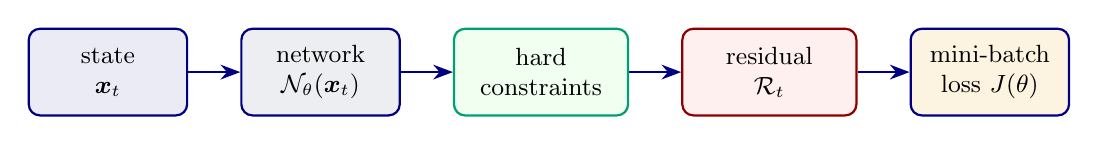
\begin{tikzpicture}[
    box/.style={rectangle, draw=uzhblue, thick, rounded corners=4pt,
                text width=1.8cm, minimum height=1.1cm, align=center, font=\small, inner sep=3pt},
    hard/.style={rectangle, draw=softgreen, thick, rounded corners=4pt,
                fill=green!6, text width=2.0cm, minimum height=1.1cm, align=center, font=\small, inner sep=3pt},
    soft/.style={rectangle, draw=darkred, thick, rounded corners=4pt,
                fill=red!6, text width=2.0cm, minimum height=1.1cm, align=center, font=\small, inner sep=3pt},
    arr/.style={-{Stealth[length=2.5mm]}, thick, uzhblue}
]
    \node[box, fill=uzhblue!8]    (x)    at ( 0.0, 0) {state\\$\state_t$};
    \node[box, fill=uzhgreylight] (nn)   at ( 2.7, 0) {network\\$\net(\state_t)$};
    \node[hard]                   (hc)   at ( 5.5, 0) {hard\\constraints};
    \node[soft]                   (res)  at ( 8.4, 0) {residual\\$\resid_t$};
    \node[box, fill=softorange!12](loss) at (11.2, 0) {mini-batch\\loss $J(\param)$};

    \draw[arr] (x)   -- (nn);
    \draw[arr] (nn)  -- (hc);
    \draw[arr] (hc)  -- (res);
    \draw[arr] (res) -- (loss);
\end{tikzpicture}
\end{center}

\vspace{0.4em}
\begin{itemize}
    \item \emphc{Hard constraints} are what the architecture can enforce exactly: budgets, positivity, market clearing.
    \item \emphc{Soft conditions} are what is left in the loss: Euler equations, KKT conditions, remaining equilibrium conditions.
    \item States are drawn from the model's own simulation, so training focuses on the ergodic set.
\end{itemize}
\end{frame}

% --- Training algorithm ---
\begin{frame}{Training Algorithm for DEQNs}
\begin{block}{Algorithm 1: Deep Equilibrium Net training}
\begin{algorithmic}
\footnotesize
\STATE \textbf{Input:} initial state $\state_0$, network $\net$, learning rate $\eta$, episodes $E$, horizon $T_{\mathrm{sim}}$, steps per episode $T_{\mathrm{train}}$
\FOR{episode $j = 1, \ldots, E$}
    \STATE \textbf{Simulate path:} $\state_0 \to \state_1 \to \cdots \to \state_{T_{\mathrm{sim}}}$ using $\net$ and the transition law, then \emphc{detach} the states
    \FOR{gradient step $m = 1, \ldots, T_{\mathrm{train}}$}
        \STATE Draw mini-batch $\mathcal{B}$ of size $B$ from $\{\state_0, \ldots, \state_{T_{\mathrm{sim}}}\}$
        \STATE $J(\param) = \frac{1}{B}\sum_{\state_i \in \mathcal{B}} \|\resid(\state_i, \net(\state_i))\|^2$
        \STATE $\param \leftarrow \param - \eta \, \nabla_\param J(\param)$
    \ENDFOR
    \STATE \textbf{Stop} when the test Euler-error quantiles stop improving over a window of episodes
\ENDFOR
\STATE \textbf{Output:} trained network $\mathcal{N}_{\param^\star}$ approximating the policy function
\end{algorithmic}
\end{block}

\vspace{0.2em}
{\footnotesize \textbf{Note.} Training points come from the \emphc{model's own simulation}, so the distribution the network is trained on \emph{moves while training}. There is no contraction here and no convergence theorem: the stopping rule has to be empirical.}
\end{frame}

% --- Where DEQNs sit ---
\begin{frame}{Where DEQNs Sit in the Literature}
\begin{columns}[T]
\column{0.48\textwidth}
\textbf{Classical global methods:}
\begin{itemize}\itemsep1pt
    \item Projection and collocation (Judd 1992)
    \item Parameterized expectations (den Haan \& Marcet 1990)
    \item Krusell \& Smith (1998)
    \item Adaptive sparse grids (Brumm \& Scheidegger 2017)
\end{itemize}

\vspace{0.4em}
\begin{exampleblock}{One sentence for macroeconomists}
\footnotesize
A DEQN is \emphc{parameterized expectations with a neural network}: the same regression on simulated data, with a flexible approximator and SGD in place of a linear projection.
\end{exampleblock}

\column{0.48\textwidth}
\textbf{Deep-learning solvers:}
\begin{itemize}\itemsep1pt
    \item \emphc{DEQNs} (Azinovic, Gaegauf \& Scheidegger 2022), this lecture
    \item Maliar, Maliar \& Winant (2021), a unified framework
    \item Duarte (2018), continuous time
    \item Fern\'andez-Villaverde et al.\ (2020), dynamic programming
    \item \emphc{DeepHAM} (Han, Yang \& E 2026), \emph{this afternoon at 15:30}
    \item Kahou et al.\ (2021), symmetry and exchangeability
\end{itemize}
\end{columns}
\end{frame}

% ============================================================================
% PART III: BROCK--MIRMAN BENCHMARK
% ============================================================================

\section{Brock--Mirman Benchmark}

\begin{frame}{}
\begin{center}
{\Huge \textcolor{uzhblue}{Part III}}\\[0.8em]
{\LARGE Brock--Mirman Benchmark}
\end{center}
\end{frame}

% --- Setup ---
\begin{frame}{Brock--Mirman (1972): Setup}
\textbf{Why this model.} It is the one growth model whose policy function is known in closed form, so every number a DEQN produces can be checked against the truth.

\vspace{0.3em}
\textbf{Planner's problem.} Choose consumption to maximize expected lifetime log utility,
\[
\max_{\{C_t\}_{t=0}^{\infty}} \; \E{\sum_{t=0}^{\infty} \beta^t \ln C_t}, \qquad
C_t + K_{t+1} \;=\; z_t K_t^{\alpha}, \qquad K_0 > 0 \text{ given},
\]
with full depreciation $\delta = 1$, capital share $\alpha \in (0,1)$, and discount factor $\beta \in (0,1)$.

\vspace{0.2em}
\textbf{Stochastic productivity.} TFP follows an AR(1) in logs, with $|\varrho| < 1$:
\[
\ln z_{t+1} \;=\; \varrho \ln z_t + \sigma_z\, \varepsilon_{t+1}, \qquad \varepsilon_{t+1} \sim \mathcal{N}(0,1).
\]

\vspace{0.2em}
\textbf{State, control, timing.} The state is $\state_t = (K_t, z_t)$ and the control is $C_t$, with $K_{t+1} = z_t K_t^\alpha - C_t$. Both $C_t$ and $K_{t+1}$ are \emphc{chosen at date $t$}, so both are measurable with respect to time-$t$ information. The network takes $(K_t, \ln z_t)$ as input.

\vspace{0.3em}
{\footnotesize That timing assumption is what lets us pull $1/C_t$ out of the expectation two slides from now.}
\end{frame}

% --- Euler equation ---
\begin{frame}{Deriving the Euler Equation (Lagrangian)}
\textbf{Step 1.} Attach a multiplier $\lambda_t$ to each period's budget:
\[
\Lag = \E{\textstyle\sum_{t=0}^{\infty} \beta^t \bigl[\ln C_t - \lambda_t( C_t + K_{t+1} - z_t K_t^{\alpha})\bigr]}.
\]

\textbf{Step 2.} $K_{t+1}$ appears \emphc{twice}, as an outflow at $t$ and through production at $t{+}1$, so both terms enter. Dividing by $\beta^t$,
\[
\frac{\partial\Lag}{\partial C_t}: \ \ \lambda_t = \frac{1}{C_t},
\qquad\qquad
\frac{\partial\Lag}{\partial K_{t+1}}: \ \ \lambda_t = \beta\,\E{\lambda_{t+1}\,\alpha z_{t+1} K_{t+1}^{\alpha-1}} .
\]

\textbf{Step 3.} As $\lambda_t$ and $K_{t+1}$ are known at $t$, iterated expectations makes the expectation conditional, and $\lambda_t = 1/C_t$ gives
\[
\boxed{\;\; \frac{1}{C_t} \;=\; \beta\, \Et{\frac{\alpha\, z_{t+1}\, K_{t+1}^{\alpha-1}}{C_{t+1}}} \;\;}
\]
{\footnotesize Marginal utility today equals discounted expected marginal utility tomorrow, times the gross marginal product of capital at $t{+}1$.}
\end{frame}

% --- Closed form ---
\begin{frame}{Closed-Form Policy via Guess-and-Verify}
\textbf{Guess.} Consumption is a constant fraction of output, $C_t = (1-s^\star)\, z_t K_t^{\alpha}$, so the budget gives $K_{t+1} = s^\star\, z_t K_t^{\alpha}$. Here $s^\star \in (0,1)$ is the \emphc{savings rate}, the object the network will learn.

\textbf{Substitute and solve.} With $C_{t+1} = (1-s^\star)\, z_{t+1} K_{t+1}^{\alpha}$ the marginal term collapses,
\[
\frac{\alpha\, z_{t+1}\, K_{t+1}^{\alpha-1}}{(1-s^\star)\, z_{t+1}\, K_{t+1}^{\alpha}}
= \frac{\alpha}{(1-s^\star)\, K_{t+1}},
\qquad\text{so}\qquad
\frac{1}{(1-s^\star) z_t K_t^{\alpha}} = \frac{\beta\alpha}{(1-s^\star) s^\star z_t K_t^{\alpha}} ,
\]
which gives $s^\star = \alpha\beta$ and therefore
\[
\boxed{\;\; C_t \;=\; (1-\alpha\beta)\, z_t K_t^{\alpha},
\qquad K_{t+1} \;=\; s^\star\, z_t K_t^{\alpha}, \qquad s^\star = \alpha\beta \;\;}
\]

{\footnotesize \emphc{Note:} $z_{t+1}$ cancels and what survives is \emph{measurable at $t$}, so $\Et{\cdot}$ passes straight through. This is special to log utility with Cobb--Douglas production and full depreciation. \ \textbf{Verify:} the Euler equation is necessary, not sufficient, and the candidate also satisfies transversality, since $\beta^t \lambda_t K_{t+1} = \alpha\beta^{t+1}/(1-\alpha\beta) \to 0$, which rules out the explosive alternatives.}
\end{frame}

% --- Hard vs soft constraints ---
\begin{frame}{Brock--Mirman: Hard vs.\ Soft Constraints}
\textbf{Split the conditions by what the architecture enforces exactly.} The network emits a savings rate through a sigmoid head, $s_t = \sigma(\net(K_t, \ln z_t))$.

\begin{center}
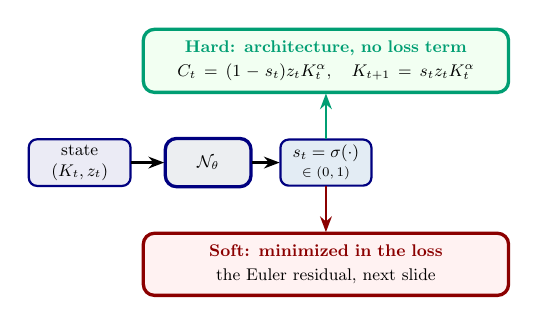
\begin{tikzpicture}[scale=0.68, transform shape,
    io/.style={rectangle, draw=uzhblue, thick, rounded corners=3pt, fill=uzhblue!8,
               minimum width=1.9cm, minimum height=0.8cm, font=\small, align=center, inner sep=3pt},
    dnn/.style={rectangle, draw=uzhblue, very thick, rounded corners=4pt, fill=uzhgreylight,
               minimum width=1.6cm, minimum height=0.9cm, font=\small\bfseries, align=center},
    sig/.style={rectangle, draw=uzhblue, thick, rounded corners=3pt, fill=softblue!15,
               minimum width=1.7cm, minimum height=0.8cm, font=\small, align=center, inner sep=3pt},
    hard/.style={rectangle, draw=softgreen, very thick, rounded corners=4pt, fill=green!5,
               text width=6.4cm, font=\small, align=center, inner sep=6pt},
    soft/.style={rectangle, draw=darkred, very thick, rounded corners=4pt, fill=red!5,
               text width=6.4cm, font=\small, align=center, inner sep=6pt},
    arr/.style={-{Stealth[length=2mm]}, thick}
]
    \node[io]  (x)  at (0,0) {state\\$(K_t,z_t)$};
    \node[dnn] (nn) at (2.4,0) {$\net$};
    \node[sig] (s)  at (4.6,0) {$s_t=\sigma(\cdot)$\\[-1pt]{\scriptsize $\in(0,1)$}};
    \draw[arr] (x)  -- (nn);
    \draw[arr] (nn) -- (s);

    \node[hard] (H) at (4.6, 1.9)
        {\textbf{\textcolor{softgreen}{Hard: architecture, no loss term}}\\[2pt]
         $C_t = (1-s_t)z_tK_t^\alpha, \quad K_{t+1} = s_t z_tK_t^\alpha$};
    \draw[arr, softgreen, thick] (s.north) -- (H.south);

    \node[soft] (S) at (4.6,-1.9)
        {\textbf{\textcolor{darkred}{Soft: minimized in the loss}}\\[2pt]
         the Euler residual, next slide};
    \draw[arr, darkred, thick] (s.south) -- (S.north);
\end{tikzpicture}
\end{center}

\begin{columns}[T]
\column{0.44\textwidth}
{\footnotesize \textbf{The resource constraint is free.} The two hard lines add to $C_t + K_{t+1} = z_tK_t^\alpha$, so it holds \emphc{identically}, for any $\param$, at every state.}

\column{0.52\textwidth}
{\footnotesize \emphc{Why a savings head?} A softplus head on $C_t$ would guarantee $C_t>0$ but could still push $K_{t+1}<0$. The sigmoid savings head removes \emph{both} failure modes before training starts. With $\delta<1$, apply the same construction to cash-on-hand.}
\end{columns}
\end{frame}

% --- The Euler residual ---
\begin{frame}{Brock--Mirman: The Euler Residual}
Write the Euler equation as a residual that vanishes exactly at the solution.
\begin{block}{Residual in consumption units, the diagnostic}
\[
e_{\mathrm{REE}} = \frac{\widehat{C}_t}{C_t} - 1, \qquad
\widehat{C}_t \equiv (u')^{-1}\bigl(\beta\,\Et{\cdot}\bigr) = \bigl(\beta\,\Et{\cdot}\bigr)^{-1},
\]
so $e_{\mathrm{REE}} = 10^{-3}$ means consumption is mispriced by \emphc{one tenth of one percent}.
\end{block}

\textbf{Tomorrow's consumption} means running the \emphc{same network again} at each shock draw:
\[
z_{t+1}(\varepsilon) = e^{\varrho \ln z_t + \sigma_z \varepsilon}, \quad
s_{t+1} = \sigma\bigl(\net(K_{t+1}, \ln z_{t+1})\bigr), \quad
C_{t+1} = (1-s_{t+1}) z_{t+1} K_{t+1}^{\alpha} ,
\]
with $K_{t+1} = s_t z_t K_t^\alpha$.

{\footnotesize \emphc{Partial depreciation.} With $\delta<1$ the marginal product becomes $\alpha z_{t+1} K_{t+1}^{\alpha-1} + (1-\delta)$, and $s^\star = \alpha\beta$ holds only at $\delta=1$.}
\end{frame}

% --- From residual to loss ---
\begin{frame}{Brock--Mirman: From Residual to Training Loss}
\textbf{Approximate the expectation first, then square.} With $Q$ quadrature nodes $\{\varepsilon_q\}$ and weights $\{w_q\}$,
\[
\resid(\state_i) \;=\; 1 \;-\; \beta\, C(\state_i) \sum_{q=1}^{Q} w_q\,
\frac{\alpha\, z_{t+1}(\varepsilon_q)\, K_{t+1}^{\alpha-1}}{C_{t+1}(\varepsilon_q)},
\qquad
\boxed{\;J(\param) \;=\; \frac{1}{N}\sum_{i=1}^{N} \bigl|\resid(\state_i)\bigr|^2\;}
\]
where $i$ indexes the $N$ simulated states in the batch.

\begin{columns}[T]
\column{0.52\textwidth}
\begin{alertblock}{Expectation inside, square outside}
\footnotesize
Replacing $\Et{\cdot}$ by a \emph{single} simulated draw and squaring that minimizes
\[
\E{e^2} \;=\; \bigl(\E{e}\bigr)^2 + \mathrm{Var}(e),
\]
whose minimizer trades bias against shock variance. It is \emph{not} the equilibrium policy.
\end{alertblock}

\column{0.46\textwidth}
\textbf{Why Brock--Mirman hides this.} Here $z_{t+1}$ cancels, so the residual is zero \emph{pathwise}, realization by realization, and both routes agree.

\vspace{0.3em}
That cancellation is knife-edge. In any model without it, the single-draw route trains the wrong object while the loss curve still looks healthy.
\end{columns}
\end{frame}

% --- Gauss-Hermite ---
\begin{frame}{Gauss--Hermite: Exact in Low Dimensions, Costly in High}
\textbf{Setup.} Shock dimension $d_\varepsilon$, with $\bm\varepsilon' \sim \mathcal{N}(0, I_{d_\varepsilon})$: Brock--Mirman has $d_\varepsilon=1$, an international real business cycle (IRBC) model with $n_c$ countries has $d_\varepsilon=n_c+1$. Gauss--Hermite uses $Q$ nodes,
\[
\E{h(\varepsilon)} \;=\; \int_{-\infty}^{\infty} h(\varepsilon)\,\frac{e^{-\varepsilon^2/2}}{\sqrt{2\pi}}\,d\varepsilon \;\approx\; \sum_{q=1}^{Q} w_q\, h(\varepsilon_q),
\]
exact for polynomials of degree $\le 2Q-1$, spectrally convergent for analytic $h$.

\begin{alertblock}{The rescaling that breaks student code}
\footnotesize
Library routines such as \texttt{numpy.polynomial.hermite.hermgauss} return the \emph{physicists'} rule, for weight $e^{-x^2}$. Convert with $\varepsilon_q = \sqrt{2}\,x_q$ and $w_q = \tilde w_q/\sqrt{\pi}$. Forgetting this gives a silently wrong expectation.
\end{alertblock}

{\footnotesize \textbf{Tensor product.} Combining one-dimensional rules costs $Q^{d_\varepsilon}$ nodes per state: for $Q=3$, $d_\varepsilon=11$, about $1.8\times 10^5$.}
\end{frame}

% --- Monomial rule ---
\begin{frame}{Stroud-3: Linear Cost in the Shock Dimension}
\textbf{Idea.} Keep exactness only to total degree $\le 3$, with nodes on the principal axes (Stroud 1957, 1971):
\[
\boxed{\;
\E{h(\bm\varepsilon')} \;\approx\; \frac{1}{2d_\varepsilon} \sum_{k=1}^{d_\varepsilon} \Bigl[\, h\bigl(+\sqrt{d_\varepsilon}\,\bm{u}_k\bigr) + h\bigl(-\sqrt{d_\varepsilon}\,\bm{u}_k\bigr)\Bigr]
\;}
\]
so $2d_\varepsilon$ nodes at radius $\sqrt{d_\varepsilon}$, with $\bm{u}_k$ the $k$-th basis vector.

\begin{columns}[T]
\column{0.50\textwidth}
{\footnotesize \textbf{The radius.} Matching the second moment, $\tfrac{1}{2d_\varepsilon}\cdot 2 r^2 = 1$, gives $r = \sqrt{d_\varepsilon}$. \ \textbf{Exact for} $\E{\varepsilon_i'} = \E{\varepsilon_i'^{\,3}} = 0$, $\E{\varepsilon_i' \varepsilon_j'} = 0$ for $i\neq j$, $\E{\varepsilon_i'^{\,2}} = 1$.}

\column{0.48\textwidth}
\begin{alertblock}{Where it stops}
\footnotesize
$\E{\varepsilon_i'^{\,4}}$ gives $d_\varepsilon$ against a truth of $3$: the fourth-moment error \emphc{grows linearly in $d_\varepsilon$}, exactly the regime the rule is used for. Check against a finer rule.
\end{alertblock}

{\footnotesize \textbf{Correlated shocks:} apply the rule to standard normals, then map through a Cholesky factor.}
\end{columns}
\end{frame}

% --- Cost comparison ---
\begin{frame}{Which Rule When}
\textbf{Per-state cost}, IRBC model with $n_c$ countries, $d_\varepsilon = n_c+1$ shocks ($Q=3$ for the tensor product):
\begin{center}
\renewcommand{\arraystretch}{1.05}
\footnotesize
\begin{tabular}{@{}rrrrl@{}}
\toprule
$n_c$ & shocks $d_\varepsilon$ & tensor product $3^{d_\varepsilon}$ & monomial $2d_\varepsilon$ & speed-up\\
\midrule
$2$  & $3$  & $27$           & $6$   & $\sim\! 5\times$\\
$5$  & $6$  & $729$          & $12$  & $\sim\! 60\times$\\
$10$ & $11$ & $177{,}147$    & $22$  & $\sim\! 8{,}000\times$\\
$20$ & $21$ & $\sim\! 10^{10}$ & $42$  & $\sim\! 2\!\times\!10^8\times$\\
\bottomrule
\end{tabular}
\end{center}

\begin{columns}[T]
\column{0.49\textwidth}
\begin{block}{Default rules of thumb}
\footnotesize
$d_\varepsilon \le 4$: Gauss--Hermite, $Q=5$. \ $5 \le d_\varepsilon \lesssim 30$: Stroud-3. \ Beyond that, or fat tails: quasi-Monte Carlo.
\end{block}

\column{0.49\textwidth}
\begin{exampleblock}{Why this is cheap to get right}
\footnotesize
Only the quadrature \emphc{kernel} changes: same loss, same training loop. Validate by tightening the rule and checking that the Euler-error histogram does not move. Degree-3 exactness usually suffices near $10^{-3}$ on IRBC-class problems (Pichler 2011; Maliar \& Maliar 2014), but that is empirical.
\end{exampleblock}
\end{columns}
\end{frame}

% --- Implementation gotchas ---
\begin{frame}{Implementation Gotchas That Cost a Day Each}
\begin{columns}[T]
\column{0.49\textwidth}
\begin{alertblock}{Detach the simulated states}
\footnotesize
The path is generated \emph{using} $\net$. If the states are not detached from the graph, autodiff differentiates through the simulation itself. Treat simulated states as fixed data, as in Azinovic et al.\ (2022).
\end{alertblock}

\begin{alertblock}{Decide about $t{+}1$ deliberately}
\footnotesize
Whether the network at $t{+}1$ carries gradient or is frozen is the target-network question from fitted value iteration. Either is defensible; silently switching between them is not.
\end{alertblock}

\column{0.49\textwidth}
\begin{block}{The rest of the checklist}
\footnotesize
\begin{itemize}\itemsep2pt
    \item \emphc{Rescale the quadrature nodes} for the probabilists' convention.
    \item \emphc{Standardize the inputs} $(K_t, \ln z_t)$ before the first layer; capital and log productivity live on very different scales.
    \item \emphc{Burn in} the simulated path before sampling from it, so training points come from the ergodic distribution and not from $\state_0$.
    \item \emphc{Evaluate the same network at every quadrature node}: $Q$ extra forward passes per state, which is the dominant cost per step.
\end{itemize}
\end{block}
\end{columns}
\end{frame}

% --- Diagnostics ---
\begin{frame}{Diagnostics: How Do We Know Training Worked?}
\textbf{Never trust a loss curve alone.} On an independent \emph{test} simulation:
\begin{enumerate}\itemsep2pt
    \item \emphc{Euler-error distribution.} Histogram $\log_{10}|e_{\mathrm{REE}}|$ on train and test states, in consumption units; both should peak near $10^{-3}$ or below, with no fatter right tail on test.
    \item \emphc{Policy-function benchmark.} Overlay the DEQN policy on the analytic $s^\star=\alpha\beta$, or on a trusted reference from time iteration or perturbation.
    \item \emphc{Ergodic-set coverage.} Scatter test states in $(K_t,\ln z_t)$: the cloud should trace the training ergodic set, neither collapsing to a point nor spreading out like a grid.
    \item \emphc{Accounting and moments.} Verify budget, market clearing and non-negativity. For heterogeneous-agent models, report \emphc{den Haan (2010)} statistics.
\end{enumerate}

\begin{alertblock}{There is no convergence theorem}
\footnotesize
Time iteration is a contraction; DEQN training is not. The sampling distribution moves as the policy moves, so ``the loss stopped falling'' proves nothing. Stop on the \emph{test} Euler-error quantiles, and report them.
\end{alertblock}
\end{frame}

% --- Validation against closed form ---
\begin{frame}{Validating a DEQN Against the Closed Form}
\begin{center}
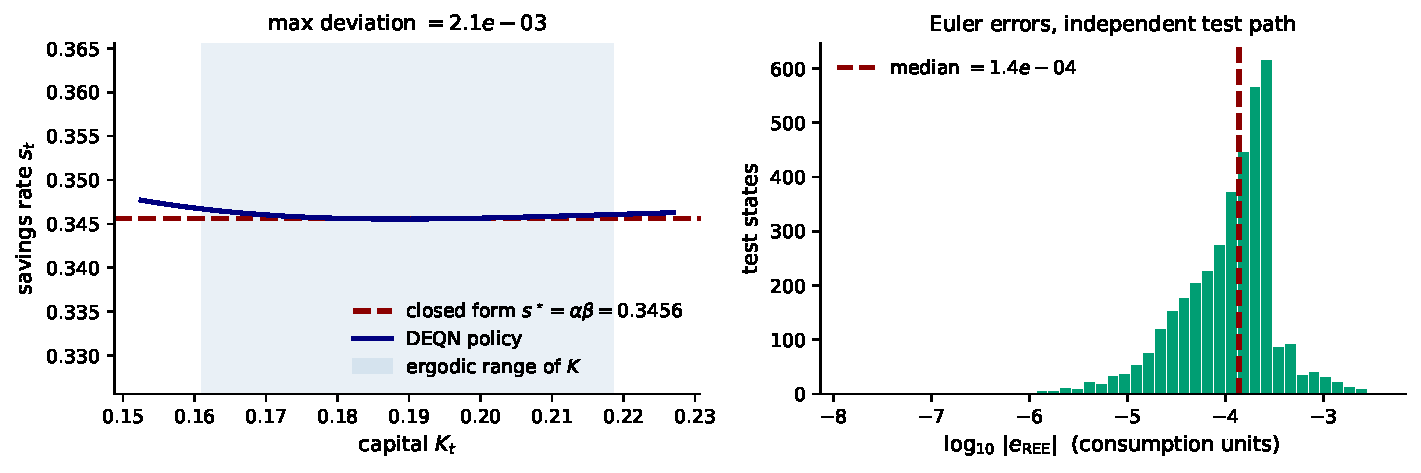
\includegraphics[height=0.53\textheight,keepaspectratio]{figures/bm_validation.pdf}
\end{center}

{\footnotesize Own computation. Stochastic Brock--Mirman, $\alpha=0.36$, $\beta=0.96$, $\varrho=0.8$, $\sigma_z=0.02$, so $s^\star=0.3456$; a $2\times 32$ tanh network with a sigmoid head, 5-node Gauss--Hermite quadrature, expectation-inside loss. \emphc{Left:} learned savings rate against the closed form. \emphc{Right:} $\log_{10}|e_{\mathrm{REE}}|$ on an independent test path. Note that the policy drifts \emph{outside} the ergodic range, where it was never trained: a preview of Part VI.}
\end{frame}

% --- Loss kernels ---
\begin{frame}{Choice of Training Loss: Six Kernels}
The loss kernel is a \emphc{modeling decision}, not a default. Write $r = \resid(\state)$ for the scalar residual at a state; same residual, same network, same data, only the reduction $r\mapsto\mathcal{L}$ changes:

\vspace{0.4em}
\begin{center}
\renewcommand{\arraystretch}{1.15}
\setlength{\tabcolsep}{4pt}
{\footnotesize
\begin{tabular}{@{}lll@{}}
\toprule
\textbf{Kernel} & \textbf{Formula} & \textbf{Character} \\
\midrule
MSE      & $\tfrac1B\sum r^2$                                & quadratic, canonical default \\
MAE      & $\tfrac1B\sum |r|$                                 & constant gradient, \emphc{stalls at small $|r|$} \\
Huber    & quadratic for $|r|\le\delta_H$, linear above       & robust hybrid, but \emphc{kink at $|r|=\delta_H$} \\
Quantile & pinball at $\tau=0.9$                              & trains the upper $\tau$-quantile only \\
CVaR     & mean of the top $10\%$ of $|r|$                    & explicitly trains the worst-case states \\
\textbf{LogCosh} & $\tfrac1B\sum\log\cosh(r)$                 & $C^\infty$: $\tfrac12 r^2$ near $0$, $|r|-\log 2$ in the tails \\
\bottomrule
\end{tabular}}
\end{center}

\vspace{0.5em}
{\footnotesize Same Brock--Mirman model with full depreciation, so $s^\star = \alpha\beta$ is in closed form; same network ($2\times32$ Swish, sigmoid head); same Adam optimizer; same training stream. Six runs differ \emph{only} in the reduction applied to the residual vector.}
\end{frame}

\begin{frame}{Loss Kernels: Convergence on Brock--Mirman}
\begin{center}
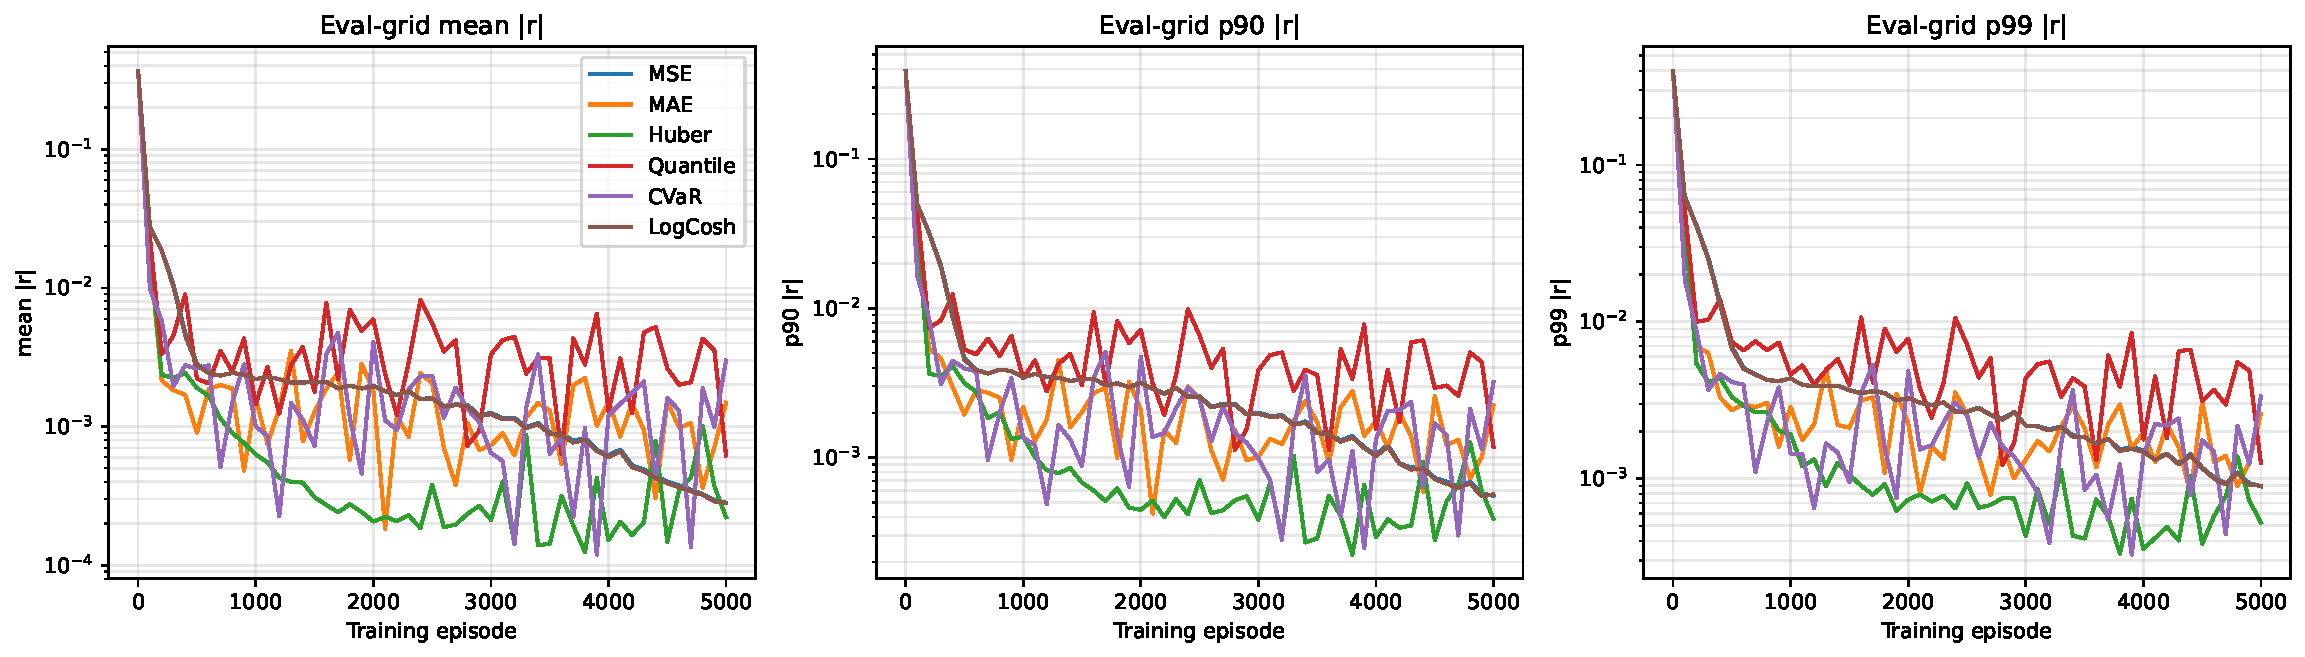
\includegraphics[height=0.40\textheight,keepaspectratio]{figures/loss_kernel_convergence.pdf}
\end{center}

\vspace{0.2em}
{\footnotesize Own computation. Mean, $p_{90}$ and $p_{99}$ of the absolute relative Euler error on a fixed evaluation grid against training episode, log scale, $5{,}000$ episodes per kernel.}

\begin{itemize}\itemsep1pt\footnotesize
    \item \emphc{LogCosh and MSE} reach the lowest mean residual here, \emphc{Huber and CVaR} the narrowest tail, and \emphc{MAE stalls} because its gradient magnitude does not shrink with the residual.
    \item This is one model with one architecture and the values are seed-sensitive. MSE stays the default; LogCosh is worth benchmarking against it; use Huber, Quantile or CVaR when the worst case matters.
    \item \emphc{Rank on the economic metric}, not the training loss: the two rankings need not agree.
\end{itemize}
\end{frame}

% --- Framing: pathologies ---
\begin{frame}{Huge Potential, but Not Yet Dynare}
\begin{itemize}\setlength\itemsep{4pt}
  \item \emphc{The promise:} grid-free, high-dimensional, kinks and all, as the benchmark confirms.
  \item \emphc{The catch:} not yet a turnkey solver, and seed-sensitive.
\end{itemize}
\begin{columns}[T,onlytextwidth]
\column{0.60\textwidth}
\textbf{\color{uzhblue}Five pathologies of self-supervised training:}
\begin{itemize}\setlength\itemsep{3pt}
  \item[(a)] \emphc{Loss-scale imbalance:} normalize and adapt the weights. \textbf{(Part IV)}
  \item[(b)] \emphc{Architecture choice:} search the candidate space. \textbf{(Part V)}
  \item[(c)] \emphc{Lazy surrogate learning:} anchors and distillation. \textbf{(Part VI)}
  \item[(d)] \emphc{Learning from scratch:} freeze a guess, learn the correction. \textbf{(Part VI)}
  \item[(e)] \emphc{Self-confirming coverage:} audit on a coverage measure. \textbf{(Part VI)}
\end{itemize}
\column{0.36\textwidth}
\begin{alertblock}{Seed dependence}
Same model, same code, different seed: one run converges and verifies, another stalls. Reproducibility is part of the method.
\end{alertblock}
\end{columns}
\end{frame}

% ============================================================================
% PART IV: LOSS BALANCING
% ============================================================================

\section{Loss Balancing}

\begin{frame}{}
\begin{center}
{\Huge \textcolor{uzhblue}{Part IV}}\\[0.8em]
{\LARGE Loss Balancing}
\end{center}
\end{frame}

% --- Motivation ---
\begin{frame}{The Residual Loss Is Not One Loss}
\textbf{Realistic economic models minimize \emph{several} residuals at once:}
\[
  J(\param)=\sum_{k=1}^{M} \omega_k\,\mathcal{L}_k(\param).
\]

\vspace{0.2cm}
\begin{columns}[T]
\column{0.50\textwidth}
\textbf{In DEQNs the components are:}
\begin{itemize}\itemsep1pt
    \item Euler equation residuals
    \item Budget constraints not enforced by the architecture
    \item Market clearing
    \item KKT and complementarity conditions
\end{itemize}

\vspace{0.25cm}
{\footnotesize The same structure appears in physics-informed neural networks, where the PDE, boundary and initial-condition residuals are separate components.}

\column{0.47\textwidth}
\begin{alertblock}{The total is not a certificate}
These components live at \emphc{vastly different scales}. With uniform weights the optimizer follows the \emphc{loudest} one and leaves quiet but economically important residuals large.\\[3pt]
A small \emph{total} loss can hide a component that is orders of magnitude too big.
\end{alertblock}
\end{columns}
\end{frame}

% --- The scale problem ---
\begin{frame}{Loss Components Differ by Orders of Magnitude}
\begin{columns}[T]
\column{0.50\textwidth}
\textbf{A three-head network.} One shared trunk, one head per residual family, one loss component each:
\[
  J(\param) = \omega_A \mathcal{L}_A + \omega_B \mathcal{L}_B + \omega_C \mathcal{L}_C .
\]

\vspace{0.2cm}
With $\mathcal{L}_A \approx 10^{0}$, $\mathcal{L}_B \approx 10^{2}$, $\mathcal{L}_C \approx 10^{4}$ and equal weights, $\mathcal{L}_C$ contributes about \emphc{$10^{4}\times$} more gradient signal than $\mathcal{L}_A$, so $\partial J/\partial\param \approx \omega_C\,\partial \mathcal{L}_C/\partial\param$ and the network effectively solves a single-task problem.

{\footnotesize This step reads the loss ratio as a gradient ratio, which requires the heads to have comparable Jacobians. GradNorm, in the appendix, drops that assumption.}

\column{0.47\textwidth}
\begin{center}
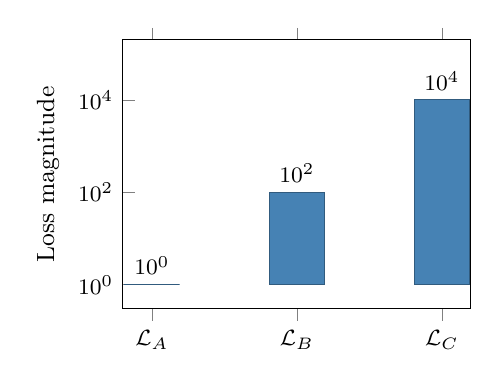
\begin{tikzpicture}
    \begin{axis}[
        ybar,
        width=6cm, height=5.0cm,
        ylabel={Loss magnitude},
        ymode=log,
        symbolic x coords={LA, LB, LC},
        xtick=data,
        xticklabels={$\mathcal{L}_A$, $\mathcal{L}_B$, $\mathcal{L}_C$},
        ymin=0.3, ymax=200000,
        bar width=20pt,
    ]
    \addplot[fill=softblue, draw=softblue!70!black] coordinates {
        (LA, 1) (LB, 100) (LC, 10000)
    };
    \node[font=\footnotesize, above] at (axis cs:LA,1) {$10^{0}$};
    \node[font=\footnotesize, above] at (axis cs:LB,100) {$10^{2}$};
    \node[font=\footnotesize, above] at (axis cs:LC,10000) {$10^{4}$};
    \end{axis}
\end{tikzpicture}\\
{\footnotesize Three loss components on a log axis}
\end{center}
\end{columns}
\end{frame}

% --- Equal weighting: dynamics ---
\begin{frame}{Equal Weighting: Training Dynamics}
\begin{center}
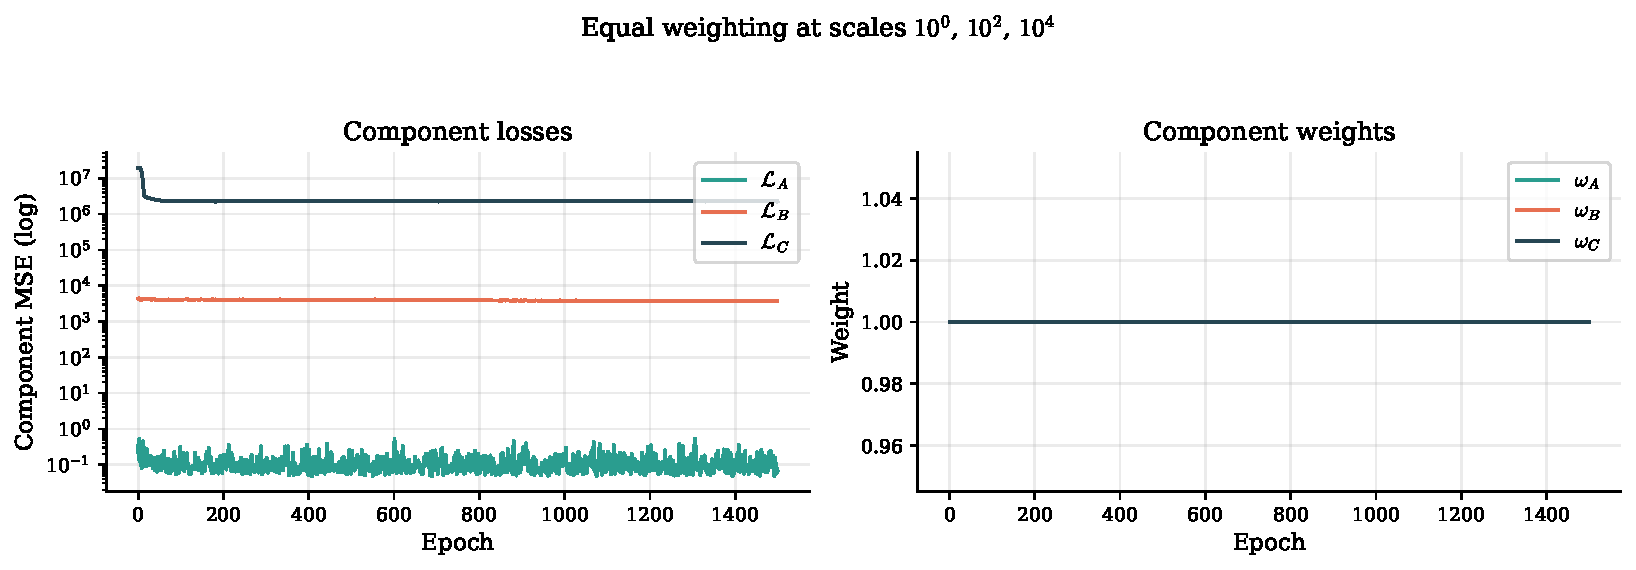
\includegraphics[height=0.46\textheight,keepaspectratio]{figures/loss_norm_equal_weights.pdf}
\end{center}

\vspace{0.2em}
{\footnotesize Own computation, notebook \texttt{02\_08}, $1{,}500$ epochs. Three Genz test functions, the standard family of tunable integrands used to benchmark approximation methods, rescaled to $10^0$, $10^2$ and $10^4$. Left: per-component mean squared error on a log axis; right: the constant component weights. $\mathcal{L}_C$ drives the gradient and converges quickly, $\mathcal{L}_B$ follows, and $\mathcal{L}_A$ is \emphc{essentially not learned}, exactly as the scale argument predicts.}
\end{frame}

% --- Non-dimensionalization ---
\begin{frame}{First, Non-Dimensionalize}
\textbf{Every residual has a natural scale.} Divide by it \emph{before} the loss sees it:
\[
  \tilde{\mathcal{L}}_k = \frac{\mathcal{L}_k}{\sigma_k^2},
  \qquad
  \sigma_k = \text{the scale of residual } k .
\]

\vspace{0.15cm}
\begin{columns}[T]
\column{0.50\textwidth}
\textbf{In a DEQN this is not a trick, it is bookkeeping:}
\begin{itemize}\itemsep1pt\footnotesize
    \item Euler errors in \emphc{consumption units}, as $e_{\mathrm{REE}}$ in Part III
    \item Budget residuals as a \emphc{share of output}
    \item Market clearing relative to the \emphc{traded quantity}
    \item Complementarity residuals relative to the \emphc{multiplier's own scale}
\end{itemize}

\vspace{0.2cm}
{\footnotesize No new hyperparameter, no schedule, no interaction with the optimizer.}

\column{0.47\textwidth}
\begin{exampleblock}{On the testbed of the next frames}
\footnotesize
Three residuals at $10^0$, $10^2$, $10^4$, five seeds, everything else held fixed. Median total relative error:
\[
  \underbrace{0.88}_{\text{equal}}
  \quad\longrightarrow\quad
  \underbrace{0.008}_{\text{non-dimensionalized}}
\]
a factor of about \emphc{$100\times$}, from a change of units.
\end{exampleblock}

\vspace{0.15cm}
{\footnotesize Adaptive weighting is what you reach for \emph{after} this step, for the imbalance that remains.}
\end{columns}
\end{frame}

% --- Inverse-loss weighting ---
\begin{frame}{Inverse-Loss Weighting}
\begin{columns}[T]
\column{0.55\textwidth}
\textbf{Idea:} weight each component in inverse proportion to its current magnitude, with exponential averaging for stability:
\begin{align*}
    \bar{\mathcal{L}}_k^{(m)} &= \beta_{\mathrm{ema}} \bar{\mathcal{L}}_k^{(m-1)} + (1 - \beta_{\mathrm{ema}}) \mathcal{L}_k^{(m)},\\
    \omega_k^{(m)} &= \frac{1}{\bar{\mathcal{L}}_k^{(m)} + 10^{-8}},
\end{align*}
then normalize so that $\sum_k \omega_k = M$. Typical choice: $\beta_{\mathrm{ema}} = 0.99$.

\vspace{0.2cm}
{\footnotesize \textbf{Hand-tuned weights} are the obvious alternative: they work only if the scales are known in advance, add $M$ hyperparameters, and go stale as the losses evolve.}

\column{0.42\textwidth}
\textbf{Pros:} simple, no hyperparameters, adapts to changing scales.

\vspace{0.2cm}
\textbf{Cons:} unstable as $\mathcal{L}_k \to 0$, weights can oscillate, no notion of \emph{relative progress}.

\vspace{0.25cm}
\begin{alertblock}{The normalization bites}
\footnotesize
Forcing $\sum_k \omega_k = M$ across losses spanning $10^8$ drives every weight but the smallest component's to \emphc{numerical zero}. On the testbed the rule ends at $\omega \approx (3, 0, 0)$: it solves the quiet residual and abandons the rest.
\end{alertblock}
\end{columns}
\end{frame}

% --- SoftAdapt ---
\begin{frame}{SoftAdapt: Weighting by Relative Progress}
\begin{columns}[T]
\column{0.54\textwidth}
\textbf{Idea} (Heydari et al., 2019): weight by \emph{relative loss changes}, so components improving slowly get more weight. With $\Delta_k^{(m)} = \mathcal{L}_k^{(m)} - \mathcal{L}_k^{(m-1)}$, rescaled to be dimensionless,
\[
\tilde\Delta_k^{(m)} = \frac{\Delta_k^{(m)}}{\mathcal{L}_k^{(m)} + 10^{-8}},
\]
\[
\hat{\omega}_k^{(m)} = M \cdot \frac{\exp\bigl(\tilde\Delta_k^{(m)} / T\bigr)}{\sum_{j} \exp\bigl(\tilde\Delta_j^{(m)} / T\bigr)} .
\]

\begin{itemize}\itemsep1pt\footnotesize
    \item $\Delta_k > 0$: the loss \emph{increased}, so it needs more weight
    \item $\Delta_k < 0$: it is already learning well
    \item $T$ is the softmax temperature: small gives winner-take-all, large gives near-equal weights
\end{itemize}

\column{0.43\textwidth}
\begin{alertblock}{Rescale before the softmax}
\footnotesize
The raw $\Delta_k$ is dimensional: a component with loss near $10^3$ produces fluctuations that swamp one near $10^{-3}$, so the softmax would react to units rather than to progress. The division above is not optional.
\end{alertblock}

\vspace{0.15cm}
{\footnotesize \textbf{Cons:} sensitive to $T$; noisy loss changes give noisy weights.}
\end{columns}
\end{frame}

% --- ReLoBRaLo idea ---
\begin{frame}{ReLoBRaLo: Relative Loss Balancing with Random Lookback}
\begin{columns}[T]
\column{0.55\textwidth}
\textbf{Three innovations} (Bischof \& Kraus, 2021):

\vspace{0.2cm}
\begin{enumerate}\itemsep4pt
    \item \textbf{Relative balancing:} use \emph{ratios} $\mathcal{L}_k^{(m)} / \mathcal{L}_k^{(m-1)}$ instead of absolute values
    \item \textbf{Baseline comparison:} mix in the \emphc{initial losses} $\mathcal{L}_k^{(0)}$ as a stable reference
    \item \textbf{Exponential smoothing:} blend new weights with history
\end{enumerate}

\column{0.42\textwidth}
\begin{block}{Why a lookback?}
\footnotesize
It prevents weight drift, resets the weights to a global perspective, and stabilizes training.
\end{block}

\vspace{0.2cm}
\begin{alertblock}{Classroom version}
\footnotesize
In the original, the baseline mix $\rho_{\mathrm{lb}}$ is a \emph{Bernoulli} draw: that randomness is the ``random lookback'' and the source of the stochastic regularization. We present the \emphc{deterministic} convex blend, which is what the exercises implement.
\end{alertblock}
\end{columns}
\end{frame}

% --- ReLoBRaLo algorithm ---
\begin{frame}{ReLoBRaLo: The Weight Update}
\begin{block}{Weight update at optimizer step $m$}
\footnotesize
\begin{algorithmic}
\STATE Compute the component losses $\mathcal{L}_1^{(m)}, \ldots, \mathcal{L}_M^{(m)}$
\STATE \textbf{Step-wise ratios:}\; $\kappa_{k,s}^{(m)}=\mathcal{L}_k^{(m)}/\bigl(T\,\mathcal{L}_k^{(m-1)}+10^{-8}\bigr)$
\STATE \textbf{Baseline ratios:}\; $\kappa_{k,b}^{(m)}=\mathcal{L}_k^{(m)}/\bigl(T\,\mathcal{L}_k^{(0)}+10^{-8}\bigr)$
\STATE $\hat \omega_{k,s}^{(m)}=M\,\operatorname{softmax}_k(\kappa_{\cdot,s}^{(m)})$, \quad
       $\hat \omega_{k,b}^{(m)}=M\,\operatorname{softmax}_k(\kappa_{\cdot,b}^{(m)})$
\STATE \textbf{Combine with smoothing:}\;
       $\omega_k^{(m)} = \alpha_{\mathrm{lb}} \bigl[\rho_{\mathrm{lb}} \, \omega_k^{(m-1)} + (1-\rho_{\mathrm{lb}}) \, \hat{\omega}_{k,b}^{(m)}\bigr] + (1-\alpha_{\mathrm{lb}}) \, \hat{\omega}_{k,s}^{(m)}$
\end{algorithmic}
\end{block}

\begin{columns}[T]
\column{0.52\textwidth}
\textbf{Which way does the weight move?} A \emph{larger} ratio $\mathcal{L}_k^{(m)}/\mathcal{L}_k^{(m-1)}$ means \emph{less} progress this step, so the softmax gives that component \emph{more} weight. The baseline term does the same against the starting point.

\column{0.44\textwidth}
\begin{exampleblock}{What the two terms buy}
\footnotesize
The step-wise ratio reacts fast but is noisy; the baseline ratio is slow but anchored. The convex blend is the compromise, and $\alpha_{\mathrm{lb}}$ decides how much of it is memory.
\end{exampleblock}
\end{columns}
\end{frame}

% --- The bound ---
\begin{frame}{How Far Can These Weights Actually Move?}
\textbf{The softmax fixes the answer before any experiment.} For any two components,
$\hat\omega_j / \hat\omega_k = \exp\bigl((\kappa_j - \kappa_k)/T\bigr)$.

\vspace{0.25cm}
\begin{columns}[T]
\column{0.52\textwidth}
The step-wise $\kappa_{k,s} = \mathcal{L}_k^{(m)}/\mathcal{L}_k^{(m-1)}$ compares \emphc{consecutive} losses, so it sits near $1$ for every component \emph{whatever its scale}; the baseline $\kappa_{k,b}$ lies in $[0,1]$.

\vspace{0.2cm}
At $T=1$ the achievable spread is therefore about $e \approx 2.7$. Measured on the testbed of the next frames: $\bm{\omega} \to (0.97,\, 1.20,\, 0.83)$, a spread of \emphc{$1.4\times$}.

\column{0.45\textwidth}
\begin{alertblock}{The consequence}
\footnotesize
A factor of $2.7$ cannot close a gap of $10^4$. ReLoBRaLo is not failing; it answers a different question. It balances \emphc{rates of progress} and is blind to \emphc{magnitude} by construction.
\end{alertblock}

\vspace{0.1cm}
{\footnotesize \textbf{Use it where it bites:} after non-dimensionalization, when one already-comparable residual converges and another stalls. That is the setting of the original paper.}
\end{columns}
\end{frame}

\begin{frame}{ReLoBRaLo: Hyperparameters}
\begin{center}
\renewcommand{\arraystretch}{1.25}
\footnotesize
\begin{tabular}{@{}c l c p{5.6cm}@{}}
\toprule
\textbf{Symbol} & \textbf{Name} & \textbf{Default} & \textbf{Effect} \\
\midrule
$T$                   & Temperature   & $1.0$   & Softmax sharpness: small is winner-take-all, large is uniform \\
$\alpha_{\mathrm{lb}}$ & Smoothing     & $0.999$ & Trust in historical weights: larger adapts more slowly \\
$\rho_{\mathrm{lb}}$   & Baseline mix  & $0.999$ & Weight on the initial-loss comparison \\
\bottomrule
\end{tabular}
\end{center}

\vspace{0.6em}
\begin{columns}[T]
\column{0.48\textwidth}
\begin{exampleblock}{Practical guidance}
The defaults work across problems. Only $T$ needs occasional tuning, and the sweep that follows shows why $T\approx 1$ is a safe starting point.
\end{exampleblock}

\column{0.48\textwidth}
{\footnotesize The subscript ``lb'' is deliberate: these are \emph{balancing} hyperparameters, and they must not be confused with the economic $\alpha$ (capital share) and the AR(1) persistence $\varrho$ from Part III.}
\end{columns}
\end{frame}

% --- ReLoBRaLo weight evolution ---
\begin{frame}{ReLoBRaLo: Weight Evolution}
\begin{center}
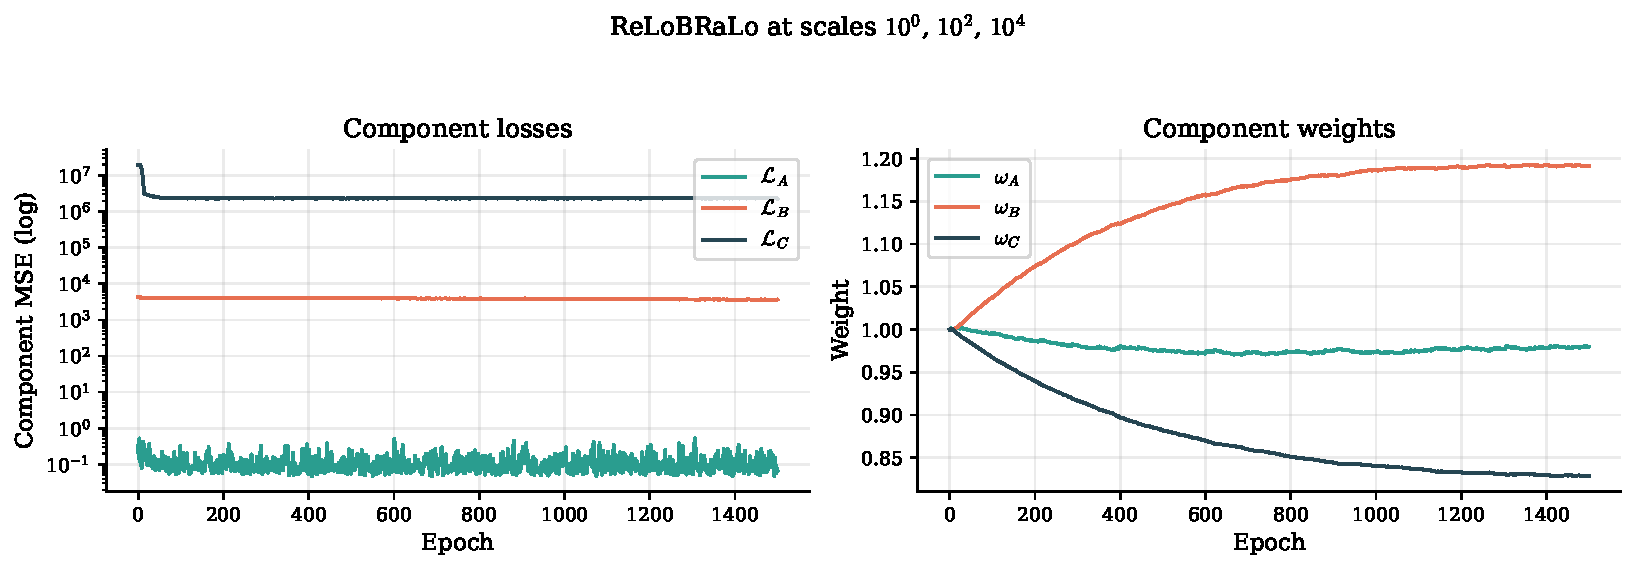
\includegraphics[height=0.46\textheight,keepaspectratio]{figures/loss_norm_relobralo_weights.pdf}
\end{center}

\vspace{0.2em}
{\footnotesize Own computation, same testbed and budget as the equal-weighting figure. Left: per-component mean squared error on a log axis under ReLoBRaLo. Right: the weight trajectories $\omega_A, \omega_B, \omega_C$. The weights move in the direction the rule intends, and they move \emphc{barely}, against a scale gap of $10^4$. The loss panel is, to the eye, the equal-weighting panel.}
\end{frame}

% --- Results ---
\begin{frame}{Results: Only One of These Is a Fix}
{\footnotesize \textbf{Testbed.} Three Genz targets on $[0,1]^2$ at scales $\sigma = 10^0, 10^2, 10^4$; shared trunk $3\times64$ ReLU with three heads; Adam with $\eta=10^{-3}$; $1{,}000$ training and $2{,}000$ test points; $1{,}500$ epochs. Score: $\sum_k \mathrm{MAE}_k/\sigma_k$. \emphc{Median over five seeds}, range in brackets.}

\vspace{0.25cm}
\begin{center}
\renewcommand{\arraystretch}{1.15}
\footnotesize
\begin{tabular}{@{}lcc@{}}
\toprule
\textbf{Rule} & \textbf{Total relative error} & \textbf{Range over seeds} \\
\midrule
Equal weights                 & $0.86$ & $[0.81,\ 0.92]$ \\
Inverse-loss weighting        & $0.42$ & $[0.38,\ 0.86]$ \\
ReLoBRaLo, $T=1$              & $0.85$ & $[0.81,\ 0.92]$ \\
ReLoBRaLo, $T=0.1$            & $0.82$ & $[0.80,\ 0.94]$ \\
\midrule
\textbf{Non-dimensionalized residuals} & \emphc{$\bm{0.008}$} & $[0.005,\ 0.008]$ \\
\bottomrule
\end{tabular}
\end{center}

\vspace{0.1cm}
\begin{itemize}\itemsep0pt\footnotesize
    \item \textbf{ReLoBRaLo sits on top of doing nothing}, exactly as the softmax bound predicts.
    \item \textbf{Inverse-loss weighting does move}, roughly halving the total, because it reacts to \emph{magnitude} --- but it gets there by abandoning two components, and it is the least stable across seeds.
    \item \textbf{Rescaling the residuals is about $\bm{110\times}$ better}, and its range overlaps nothing.
\end{itemize}
\end{frame}

% --- T sensitivity ---
\begin{frame}{Sensitivity to the Temperature $T$}
\begin{columns}[T]
\column{0.55\textwidth}
\begin{center}
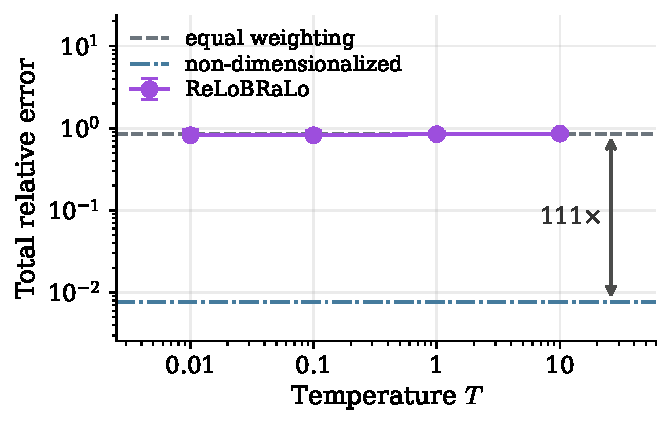
\includegraphics[height=4.2cm,keepaspectratio]{figures/loss_norm_T_sensitivity.pdf}
\end{center}
{\footnotesize Own computation. Total relative error at the end of training, swept over $T$, against the two reference levels. Keep $T \approx 1$ and spend the tuning effort on the units instead.}

\column{0.42\textwidth}
\textbf{What $T$ controls} is the spread $\exp(\Delta\kappa/T)$ of the previous frame: small $T$ buys authority at the price of winner-take-all behavior, large $T$ collapses to equal weights.

\vspace{0.25cm}
\begin{alertblock}{What the sweep shows}
\footnotesize
\emphc{No temperature closes the gap.} All four medians sit on the equal-weighting line, two orders of magnitude above the non-dimensionalized one, and the error bars show how little separates them.
\end{alertblock}
\end{columns}
\end{frame}

% --- Loss normalization summary ---
\begin{frame}{Loss Balancing in DEQNs: What to Remember}
\begin{columns}[T]
\column{0.55\textwidth}
\textbf{Takeaways:}
\begin{enumerate}\itemsep2pt\small
    \item Multi-component losses at different scales cause \emphc{gradient dominance}.
    \item \textbf{Non-dimensionalize first.} Free, no hyperparameter, worth about $100\times$ here: Euler errors in consumption units, budget residuals as a share of output.
    \item Inverse-loss weighting is \emphc{not} a scale fix: $\sum_k \omega_k = M$ collapses the weights onto the quietest component.
    \item \textbf{ReLoBRaLo} balances \emph{relative progress}, and its softmax can only spread the weights by about $e^{1/T}$. Use it \emph{after} step 2.
    \item \emphc{Monitor every component separately}, in scale-free units.
\end{enumerate}

\column{0.42\textwidth}
\begin{exampleblock}{Remedy}
Rescale each residual by its own natural scale. Only then reach for adaptive weighting, and report per-component residuals rather than the total.
\end{exampleblock}

\vspace{0.2cm}
{\footnotesize \textbf{References:} Bischof \& Kraus (2021, arXiv:2110.09813; \emph{CMAME} 439, 2025), ReLoBRaLo; Heydari et al.\ (2019), SoftAdapt; Chen et al.\ (2018), GradNorm; Wang, Teng \& Perdikaris (2021), gradient-flow pathologies in PINNs.}
\end{columns}
\end{frame}

% ============================================================================
% PART V: ARCHITECTURE SEARCH
% ============================================================================

\section{Architecture Search}

\begin{frame}{}
\begin{center}
{\Huge \textcolor{uzhblue}{Part V}}\\[0.8em]
{\LARGE Architecture Search}
\end{center}
\end{frame}

% --- Architecture is part of the numerical method ---
\begin{frame}{Architecture Is Part of the Numerical Method}
\begin{columns}[T,onlytextwidth]
\column{0.54\textwidth}
\textbf{\color{uzhblue}Symptom.} With the \emph{same} equations, one network converges and another stalls. Width, depth, activation and learning rate are \emphc{numerical-method choices}, not cosmetics.

\vspace{0.4em}
\textbf{\color{uzhblue}Why this matters in economics:}
\begin{itemize}\setlength\itemsep{3pt}\footnotesize
  \item \textbf{DSGE policy functions:} search improves convergence on the \emph{same} model.
  \item \textbf{Surrogates:} when a network replaces a costly simulation, architecture sets approximation quality.
  \item \textbf{Reproducibility:} a search records which architectures were tried.
\end{itemize}

\column{0.42\textwidth}
\begin{center}
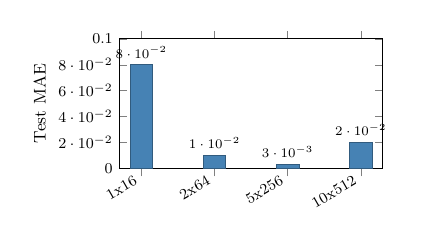
\begin{tikzpicture}[scale=0.68, transform shape]
    \begin{axis}[
        ybar,
        width=6.5cm, height=4.0cm,
        ylabel={Test MAE},
        symbolic x coords={1x16, 2x64, 5x256, 10x512},
        xtick=data,
        x tick label style={rotate=30, anchor=east},
        ymin=0, ymax=0.1,
        bar width=12pt,
        nodes near coords,
        every node near coord/.append style={font=\scriptsize},
        nodes near coords align={vertical},
    ]
    \addplot[fill=softblue, draw=softblue!70!black] coordinates {
        (1x16, 0.08) (2x64, 0.01) (5x256, 0.003) (10x512, 0.02)
    };
    \end{axis}
\end{tikzpicture}\\
{\footnotesize Own computation. Four architectures, same data: the test MAE moves by an order of magnitude.}
\end{center}

\begin{alertblock}{Hand-tuning does not scale}
\footnotesize
One architecture is one experiment. Reporting only the winner hides how fragile the result is.
\end{alertblock}
\end{columns}
\end{frame}

% --- The hyperparameter space ---
\begin{frame}{The Hyperparameter Space}
\begin{columns}[T]
\column{0.50\textwidth}
\textbf{Architectural hyperparameters:}
\begin{itemize}
    \item Hidden layers $L \in \{1, \ldots, 5\}$
    \item Units per layer in $\{32, 64, 96, \ldots, 256\}$, 8 values in steps of 32
    \item Activation: ReLU, tanh, Swish
\end{itemize}

\vspace{0.3cm}
\textbf{Training hyperparameters:}
\begin{itemize}
    \item Learning rate log-uniform on $[10^{-4}, 10^{-2}]$, on a 20-point grid
    \item Batch size $B \in \{64, 128, 256\}$
    \item Epochs, regularization, \ldots
\end{itemize}

\column{0.47\textwidth}
\begin{block}{Combinatorial explosion}
Even this modest search space has
\[
    |\mathcal{H}| = 5 \times 8 \times 3 \times 20 \times 3 = \emphc{7{,}200}
\]
configurations, before epochs and regularization are added.
\begin{itemize}
    \item Each trial: minutes to hours
    \item Full grid: \emphc{infeasible}
\end{itemize}
\end{block}

\vspace{0.3cm}
{\footnotesize \textbf{``Grad-student descent''} (pick, train, adjust one thing, repeat until the deadline) \emphc{does not scale}, embeds human bias, and is not reproducible.}
\end{columns}
\end{frame}

% --- Grid and random search ---
\begin{frame}{Grid Search and Random Search}
\begin{columns}[T]
\column{0.46\textwidth}
\textbf{Grid search.} Enumerate all combinations on a regular grid. Cost $\mathcal{O}(k^{d_h})$, exponential in the number $d_h$ of hyperparameters. Embarrassingly parallel, but it spends most of the budget on axes that do not matter.

\vspace{0.3cm}
\textbf{Random search.} Sample configurations uniformly at random.

\vspace{0.15cm}
\emphc{The result} (Bergstra \& Bengio, 2012): when only a \emph{few} dimensions matter, random search needs \emph{fewer} trials, because each trial contributes a fresh value on every axis.

\column{0.52\textwidth}
\begin{center}
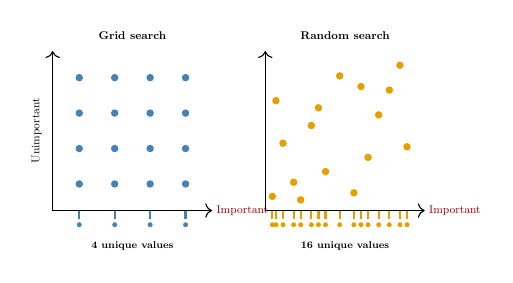
\begin{tikzpicture}[scale=0.45, transform shape]
    \begin{scope}[shift={(0,0)}]
        \draw[->] (0,0) -- (4.5,0) node[right,font=\small] {\emphc{Important}};
        \draw[->] (0,0) -- (0,4.5);
        \node[font=\small, rotate=90] at (-0.45,2.25) {Unimportant};
        \foreach \xi in {0.75,1.75,2.75,3.75} {
            \foreach \yi in {0.75,1.75,2.75,3.75} {
                \fill[softblue] (\xi,\yi) circle (3pt);
            }
        }
        \foreach \xi in {0.75,1.75,2.75,3.75} {
            \draw[softblue, thick, dashed] (\xi,0) -- (\xi,-0.4);
            \fill[softblue] (\xi,-0.4) circle (2pt);
        }
        \node[font=\footnotesize] at (2.25,-1.0) {\textbf{4 unique values}};
        \node[font=\small, above] at (2.25,4.7) {\textbf{Grid search}};
    \end{scope}

    \begin{scope}[shift={(6.0,0)}]
        \draw[->] (0,0) -- (4.5,0) node[right,font=\small] {\emphc{Important}};
        \draw[->] (0,0) -- (0,4.5);
        \fill[softorange] (0.3,3.1) circle (3pt);
        \fill[softorange] (0.8,0.8) circle (3pt);
        \fill[softorange] (1.3,2.4) circle (3pt);
        \fill[softorange] (1.7,1.1) circle (3pt);
        \fill[softorange] (0.5,1.9) circle (3pt);
        \fill[softorange] (2.1,3.8) circle (3pt);
        \fill[softorange] (2.5,0.5) circle (3pt);
        \fill[softorange] (2.9,1.5) circle (3pt);
        \fill[softorange] (3.2,2.7) circle (3pt);
        \fill[softorange] (3.5,3.4) circle (3pt);
        \fill[softorange] (3.8,4.1) circle (3pt);
        \fill[softorange] (1.0,0.3) circle (3pt);
        \fill[softorange] (1.5,2.9) circle (3pt);
        \fill[softorange] (0.2,0.4) circle (3pt);
        \fill[softorange] (2.7,3.5) circle (3pt);
        \fill[softorange] (4.0,1.8) circle (3pt);
        \foreach \xi in {0.2,0.3,0.5,0.8,1.0,1.3,1.5,1.7,2.1,2.5,2.7,2.9,3.2,3.5,3.8,4.0} {
            \draw[softorange, thick, dashed] (\xi,0) -- (\xi,-0.4);
            \fill[softorange] (\xi,-0.4) circle (2pt);
        }
        \node[font=\footnotesize] at (2.25,-1.0) {\textbf{16 unique values}};
        \node[font=\small, above] at (2.25,4.7) {\textbf{Random search}};
    \end{scope}
\end{tikzpicture}
\end{center}

\vspace{0.15cm}
{\footnotesize Same 16 evaluations: the grid wastes most on the unimportant axis. \textbf{The condition does the work:} with one relevant axis the median best-found value improves by $13\times$ at $d_h=2$ and $10^3\times$ at $d_h=8$, but that edge \emphc{disappears} once the spare axes carry a tenth of the objective, and at $d_h=1$ the grid wins.}
\end{columns}
\end{frame}

% --- Hyperband ---
\begin{frame}{Hyperband and Successive Halving}
\begin{columns}[T]
\column{0.44\textwidth}
\textbf{Idea:} start many configurations cheaply, \emphc{stop the worst early}, give the survivors more resources. Successive halving (Karnin et al.\ 2013; Jamieson \& Talwalkar 2016) keeps the top $1/\gamma$ and multiplies the budget by $\gamma$, so \emph{every round costs the same}.

\vspace{0.3cm}
\textbf{Hyperband} (Li et al., 2018) runs successive halving with several brackets, hedging across the unknown correlation between early and late performance. \emph{BOHB} (Falkner et al., 2018) replaces the random sampling with Bayesian optimization.

\column{0.54\textwidth}
\begin{center}
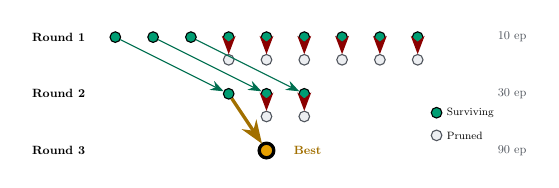
\begin{tikzpicture}[scale=0.48, transform shape,
    trialnode/.style={circle, draw, minimum size=8pt, inner sep=0pt},
    alive/.style={trialnode, fill=softgreen},
    dead/.style={trialnode, fill=uzhgreylight, draw=uzhgreydark},
    >=Stealth,
]
    \node[font=\small\bfseries] at (-1.5, 0) {Round 1};
    \node[font=\small\bfseries] at (-1.5,-1.5) {Round 2};
    \node[font=\small\bfseries] at (-1.5,-3.0) {Round 3};

    \node[font=\small, uzhgreydark] at (10.5, 0) {10 ep};
    \node[font=\small, uzhgreydark] at (10.5,-1.5) {30 ep};
    \node[font=\small, uzhgreydark] at (10.5,-3.0) {90 ep};

    \foreach \i in {0,...,8} {
        \node[alive] (r1-\i) at (\i*1.0, 0) {};
    }
    \foreach \i in {0,...,2} {
        \node[alive] (r2-\i) at (\i*1.0 + 3.0, -1.5) {};
    }
    \foreach \i in {3,...,8} {
        \node[dead] (r1d-\i) at (\i*1.0, -0.6) {};
        \draw[->, darkred, thick] (r1-\i) -- (r1d-\i);
    }
    \draw[->, softgreen!70!black] (r1-0) -- (r2-0);
    \draw[->, softgreen!70!black] (r1-1) -- (r2-1);
    \draw[->, softgreen!70!black] (r1-2) -- (r2-2);

    \node[alive, fill=softorange, minimum size=11pt, line width=1.2pt] (r3-0) at (4.0, -3.0) {};
    \foreach \i in {1,2} {
        \node[dead] (r2d-\i) at (\i*1.0 + 3.0, -2.1) {};
        \draw[->, darkred, thick] (r2-\i) -- (r2d-\i);
    }
    \draw[->, softorange!70!black, line width=1.2pt] (r2-0) -- (r3-0);
    \node[font=\small\bfseries, softorange!70!black, right] at (4.6,-3.0) {Best};

    \node[alive, label={right:\footnotesize Surviving}] at (8.5, -2.0) {};
    \node[dead, label={right:\footnotesize Pruned}] at (8.5, -2.6) {};
\end{tikzpicture}
\end{center}

\vspace{0.2cm}
{\footnotesize Cascade $9 \to 3 \to 1$ at $\gamma=3$. Each round costs $9\cdot10 = 3\cdot30 = 1\cdot90 = 90$ epoch-equivalents, so the total is $\emphc{270}$ against $810$ for training all nine configurations fully.}
\end{columns}
\end{frame}

% --- Search results ---
\begin{frame}{Search Results: Random Search vs.\ Successive Halving}
{\footnotesize \textbf{Testbed.} Two-dimensional Genz Gaussian, $1{,}000$ training and $2{,}000$ test points; search over layers $1$--$5$, units $32$--$256$, activation in \{ReLU, tanh, Swish\}, learning rate in $[10^{-4},10^{-2}]$; baseline $3\times64$ ReLU.}

\vspace{0.2cm}
\begin{center}
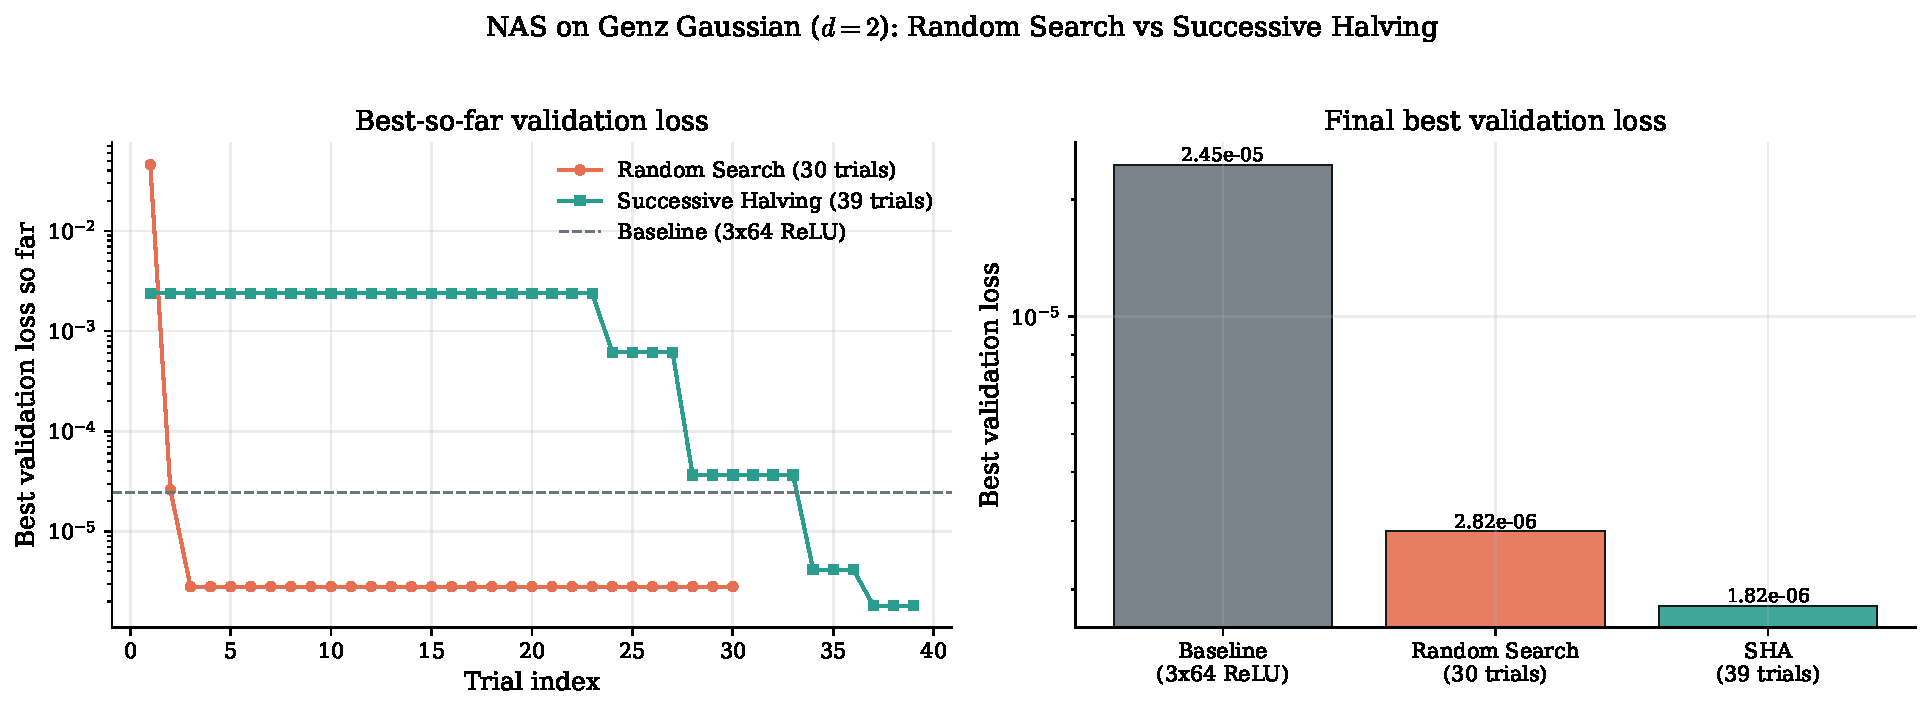
\includegraphics[height=0.44\textheight,keepaspectratio]{figures/nas_search_results.pdf}
\end{center}

\vspace{0.2em}
{\footnotesize Own computation. Random search uses $30$ full trials; successive halving uses $27$ initial candidates at $\gamma=3$. Both reach a test MAE of order $10^{-3}$ from a baseline near $4\cdot10^{-3}$, and successive halving needs about $2.3\times$ less configuration-epoch budget in this seeded run.}
\end{frame}

% --- Best model vs ground truth ---
\begin{frame}{Best Model vs.\ Ground Truth}
\begin{center}
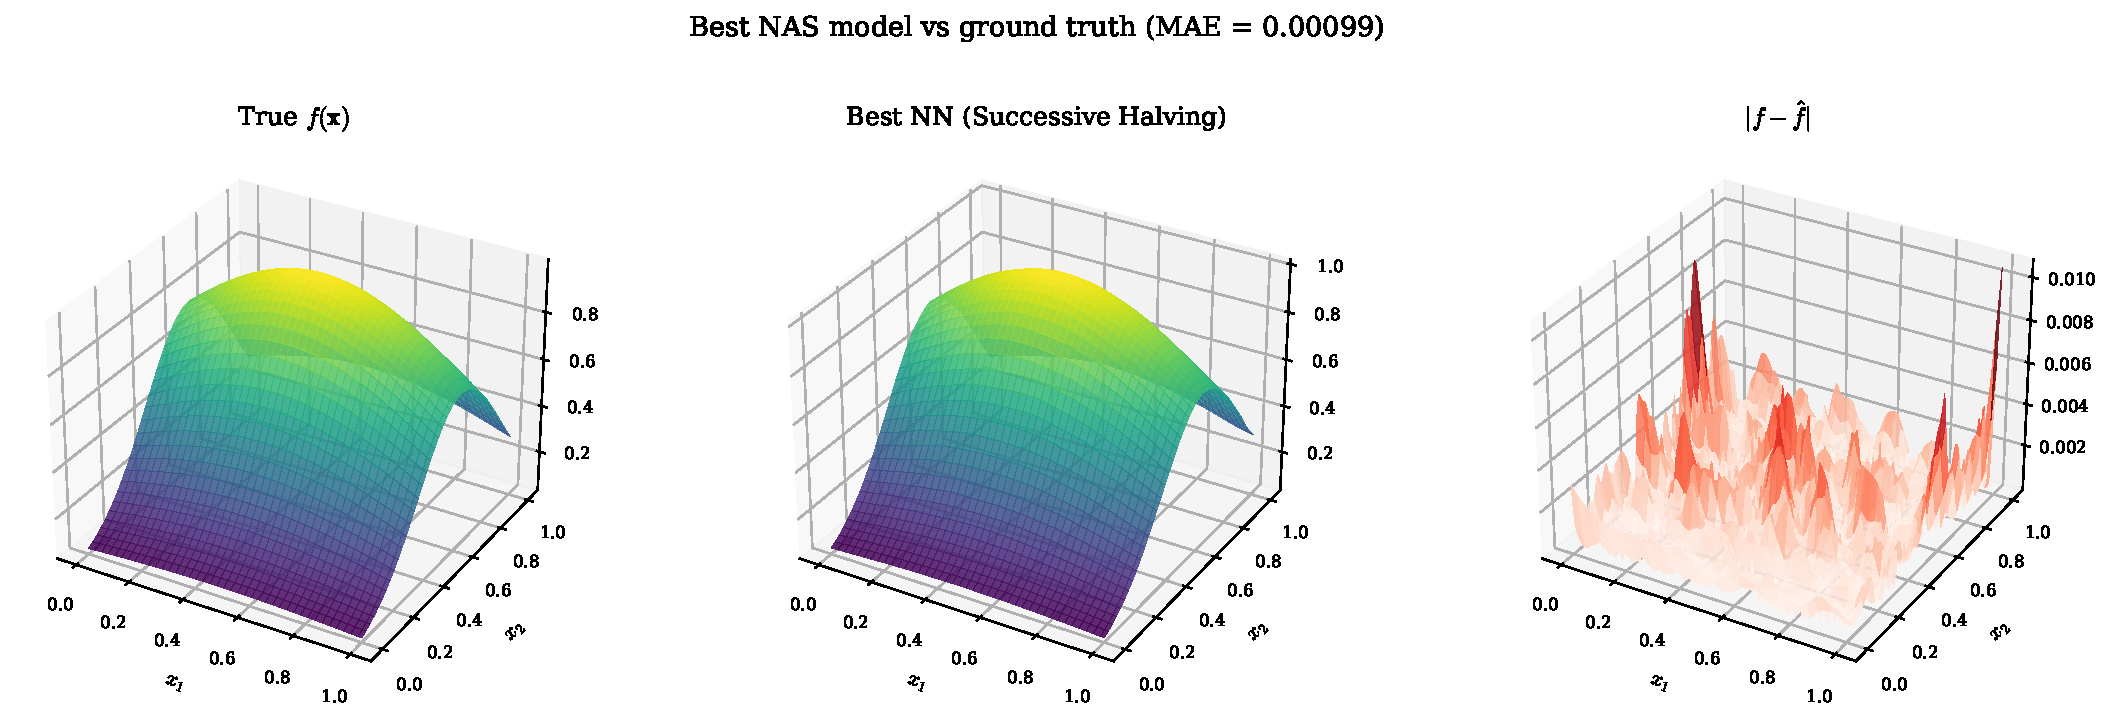
\includegraphics[height=0.50\textheight,keepaspectratio]{figures/nas_best_surface.pdf}
\end{center}

\vspace{0.2em}
{\footnotesize Own computation. Left to right: the true Genz target, the best network found by the search, and the absolute error map on $[0,1]^2$. On this two-dimensional test function, and before the economic model changed at all, architecture search moved the validation loss by more than an order of magnitude.}
\end{frame}

% --- Best practices ---
\begin{frame}{Architecture Search in Practice}
\begin{columns}[T]
\column{0.48\textwidth}
\textbf{Search space design:}
\begin{itemize}\itemsep2pt
    \item Start small, expand if needed
    \item Use a \emphc{log scale} for the learning rate
    \item Include the current best configuration as a candidate
\end{itemize}

\vspace{0.35cm}
\textbf{Budget allocation:}
\begin{itemize}\itemsep2pt
    \item Returns diminish once the space has been explored, often after a few tens of trials
    \item Hyperband: the default reduction factor $\gamma = 3$ is a reasonable start
    \item Fix the \emphc{compute budget up front}
\end{itemize}

\column{0.48\textwidth}
\textbf{Common pitfalls:}
\begin{itemize}\itemsep2pt
    \item Search space too large, so the budget is wasted
    \item Overfitting the validation set, so keep a holdout test set
    \item Ignoring training stability, so check the learning curves too
\end{itemize}

\vspace{0.4cm}
\begin{exampleblock}{Remedy}
Report the candidate space and the protocol, not only the winner.
\end{exampleblock}
\end{columns}
\end{frame}

% ============================================================================
% PART VI: FURTHER PATHOLOGIES, HPC, WRAP-UP
% ============================================================================

\section{Further Pathologies, HPC, and Wrap-Up}

\begin{frame}{}
\begin{center}
{\Huge \textcolor{uzhblue}{Part VI}}\\[0.8em]
{\LARGE Further Pathologies, HPC, and Wrap-Up}
\end{center}
\end{frame}

\begin{frame}{Three Pathologies Left}
\begin{columns}[T]
\column{0.52\textwidth}
\textbf{Where we are:}
\begin{itemize}\setlength\itemsep{4pt}
  \item[(a)] Loss-scale imbalance \hfill \textcolor{softgreen}{\textbf{done, Part IV}}
  \item[(b)] Architecture choice \hfill \textcolor{softgreen}{\textbf{done, Part V}}
  \item[(c)] \emphc{Lazy surrogate learning}
  \item[(d)] \emphc{Learning from scratch}
  \item[(e)] \emphc{Self-confirming coverage}
\end{itemize}

\vspace{0.6em}
The last three share a feature: the loss looks fine while the policy is wrong. None of them is visible on a training curve.

\column{0.44\textwidth}
\begin{alertblock}{The common thread}
Residual-only training measures the policy \emph{where the policy itself decides to look}. Every remedy in this part changes \emph{what is measured}, not the economics.
\end{alertblock}

\vspace{0.4em}
{\footnotesize After the pathologies: data parallelism, the hands-on preview, and the wrap-up.}
\end{columns}
\end{frame}

% ---- (c) lazy surrogate learning ----
\begin{frame}{Lazy Learning: Low Residual, Wrong Policy}
\begin{columns}[T,onlytextwidth]
\column{0.46\textwidth}
\begin{itemize}\setlength\itemsep{4pt}
  \item \textbf{\color{uzhblue}Symptom.} Lazy training is a typical pitfall of \emphc{self-supervised} (residual-only) learning: it drives the equilibrium residual down while the policy stays inaccurate across the state and parameter domain.
  \item Fix a state and vary a \emph{parameter} $\psi$: a taste, a tax, or a shock size.
  \item The true policy moves with $\psi$; the lazy surrogate stays \emph{flat}, so it gets the level right on average and the \emphc{sensitivity} wrong.
\end{itemize}
\column{0.52\textwidth}
\centering
\begin{tikzpicture}
\begin{axis}[width=\linewidth,height=0.58\textheight,
   xlabel={parameter $\psi$},ylabel={policy at a fixed state},
   xmin=0,xmax=1,ymin=0,ymax=1.3,
   axis lines=left, clip=false]
 \addplot[uzhblue,very thick,domain=0:1,samples=60]{0.12+0.62*x+0.22*x*x};
 \node[uzhblue,font=\footnotesize\bfseries,anchor=east]
   at (axis cs:0.98,1.04){true $p^\star(\psi)$};
 \addplot[harvardcrimson,very thick,densely dashed,domain=0:1,samples=2]{0.50+0.04*x};
 \node[harvardcrimson,font=\footnotesize\bfseries,anchor=north east]
   at (axis cs:0.97,0.47){lazy $\net(\psi)$};
 \draw[<->,thick,uzhgreydark] (axis cs:0.85,0.55) -- (axis cs:0.85,0.79);
 \node[uzhgreydark,font=\footnotesize,anchor=south] at (axis cs:0.55,1.14){missed $\psi$-dependence};
\end{axis}
\end{tikzpicture}\\[2pt]
{\footnotesize At a fixed state the true policy varies with $\psi$ (blue), while the lazy surrogate is almost flat (red dashed). The loss is low and the parameter dependence is weak: the mask is convincing only on average.}
\end{columns}
\end{frame}

\begin{frame}{The Fix: Anchors and Distillation}
\vspace*{\fill}
\begin{columns}[T,onlytextwidth]
\column{0.56\textwidth}
\textbf{Fix.} Augment the self-supervised residual with a small \emphc{semi-supervised distillation} term on a few trusted anchor states:
\[
  J^{\mathrm{dist}}(\param)=J(\param)
   +\lambda_{\mathrm{a}}\!\sum_{\state_a\in\mathcal A}\!\bigl\|\net(\state_a)-p^\star(\state_a)\bigr\|^2 .
\]
\begin{itemize}\setlength\itemsep{3pt}
  \item $\mathcal A$: a handful of anchor states.
  \item $p^\star$: reference policies from an accurate solver, such as perturbation, a low-dimensional solve, or a converged reference run.
  \item $\lambda_{\mathrm{a}}$ is one more weight, so Part IV applies to it as well.
\end{itemize}
\column{0.40\textwidth}
\begin{exampleblock}{Remedy}
\footnotesize
In the deep uncertainty-quantification application of Friedl et al.\ (2023), about \emphc{10 to 20 anchors} are typically enough to stabilize training, and leave-one-out diagnostics show the distilled surrogate agreeing with the reference policies to \emphc{within one percent}.
\end{exampleblock}
\end{columns}
\vspace*{\fill}
\end{frame}

% ---- (d) residual learning ----
\begin{frame}{Residual Learning: Freeze and Correct}
\begin{columns}[T,onlytextwidth]
\column{0.50\textwidth}
\textbf{Idea.} Do not ask the network for the \emph{whole} solution, only for the \emphc{correction} to a cheap baseline:
\[
  p(\state)=\underbrace{p_0(\state)}_{\text{frozen guess}}
   +\;\net(\state).
\]
\begin{itemize}\setlength\itemsep{3pt}\footnotesize
  \item $p_0$: a cheap guess (steady state, perturbation, certainty equivalent).
  \item The network learns only the \emph{small, nonlinear} part, which is easier than the level and the shape at once.
  \item The solution is sane from iteration zero, which matters when a bad start diverges.
  \item $\rightarrow$ \emphc{The network is a proofreader, not an author.}
\end{itemize}
\column{0.48\textwidth}
\centering
\begin{tikzpicture}
\begin{axis}[width=\linewidth,height=0.56\textheight,
   xlabel={state},xmin=0,xmax=3,ymin=-0.5,ymax=2.7,
   axis line style={uzhgreydark},ytick=\empty,
   legend style={draw=uzhgreydark!40,at={(0.02,0.98)},
                 anchor=north west,row sep=-1pt}]
  \addplot[uzhgreydark,thick,dashed,domain=0:3,samples=40]{0.6*x+0.45};
  \addlegendentry{frozen $p_0$ (perturbation)}
  \addplot[harvardcrimson,very thick,domain=0:3,samples=160]
    {0.6*x+0.45+0.30*sin(deg(110*x))};
  \addlegendentry{true policy}
  \addplot[softgreen!80!black,very thick,domain=0:3,samples=160]
    {0.30*sin(deg(110*x))};
  \addlegendentry{$\net$: the correction}
\end{axis}
\end{tikzpicture}\\[2pt]
{\footnotesize The network only fits the small wiggle: frozen guess plus learned correction.}
\end{columns}
\end{frame}

% ---- (e) coverage ----
\begin{frame}{Residual Training Only Tests States the Policy Visits}
Every DEQN solver is \emphc{self-supervised}: it drives an equation residual to zero on the states its \emph{own} policy generates,
\[
  J(\param)=
  \mathbb{E}_{\state\sim\mu_{\param}}
  \bigl\|\,\resid\!\left(\state,\net(\state)\right)\bigr\|^2 ,
\]
so the sampling measure $\mu_{\param}$ is generated \emphc{by the candidate policy itself}.

\vspace{0.6em}
\begin{itemize}\setlength\itemsep{5pt}
  \item The residual is only ever tested where the current policy already goes.
  \item A low loss says \emphc{nothing} about the states the policy avoids.
  \item A wrong policy visits the wrong states, so the error \emphc{hides exactly where it is never measured}.
  \item The loss \emphc{confirms itself}: a property of residual-only training, shared by every method in this lecture, and not a DEQN-specific flaw.
\end{itemize}
\end{frame}

\begin{frame}{Equilibrium World Models: A Disciplined Dreamer}
{\footnotesize \emphc{Equilibrium World Models} (EWM) keep the economics, changing \emphc{where} the residual is imposed.}
\begin{center}
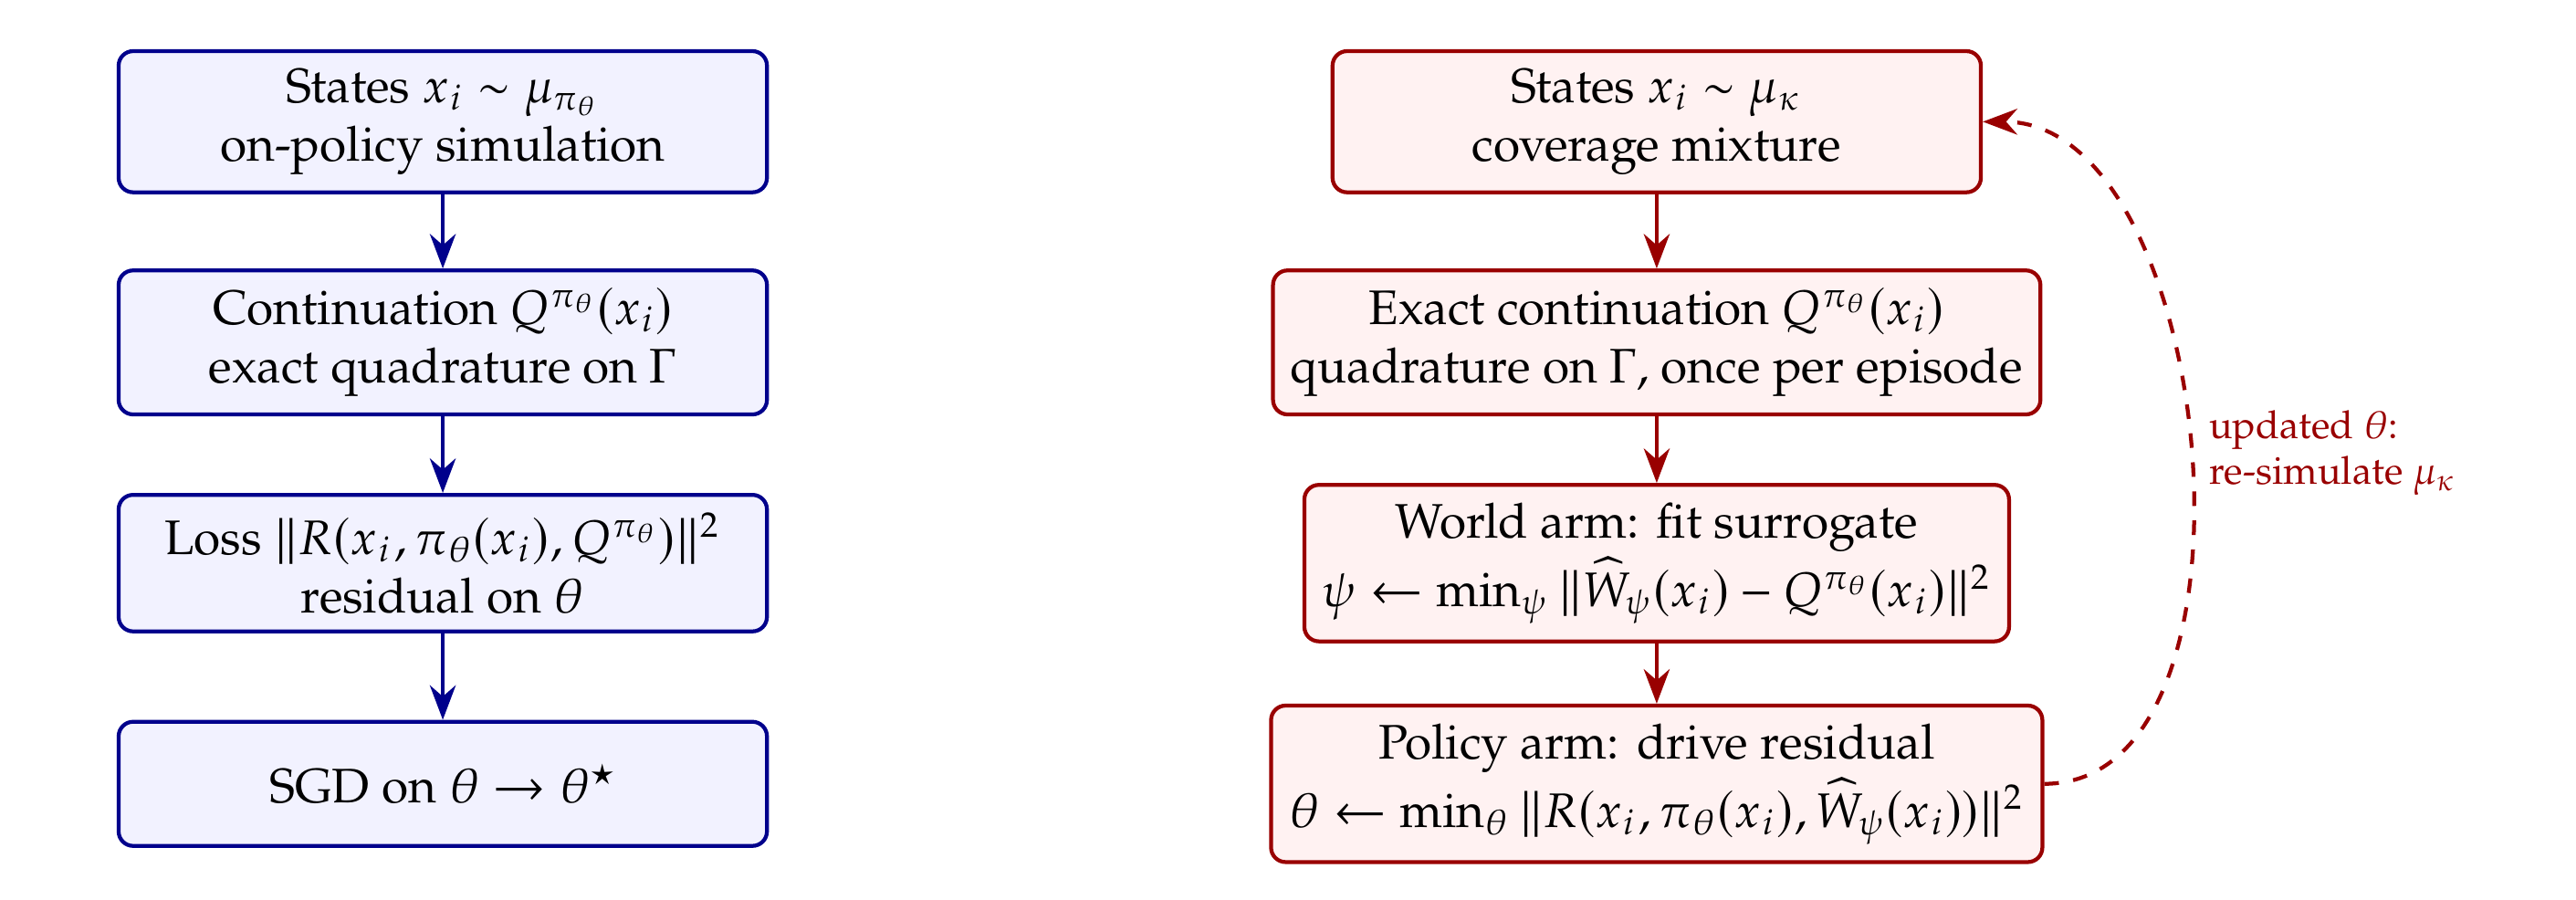
\includegraphics[height=0.36\textheight,keepaspectratio]{figures/ewm_mechanism.png}
\end{center}
{\footnotesize Left: an ordinary residual solver, measuring along its own path. Right: EWM, measuring on a broader coverage measure. Schaab \& Scheidegger (2026), work in progress; Dreamer lineage: Ha \& Schmidhuber (2018), Hafner et al.\ (2023).}
\vspace{-0.2em}

\vspace{0.2em}
\begin{columns}[T]
\column{0.49\textwidth}
{\footnotesize \emphc{New:} a coverage measure $\cov=c_1\mu_{\param}+c_2\mu^{\mathrm{stress}}+c_3\mu^{\mathrm{local}}$ and a learned continuation value, so the residual can be evaluated off-path.}

\column{0.49\textwidth}
{\footnotesize \emphc{Unchanged:} the law of motion and the residual. The audit is stronger because it runs on $\cov$, not because the economics changed.}
\end{columns}
\end{frame}

\begin{frame}{What the Audit Buys: Off-Path Credibility}
\begin{columns}[T,onlytextwidth]
\column{0.50\textwidth}
\centering\sloppy
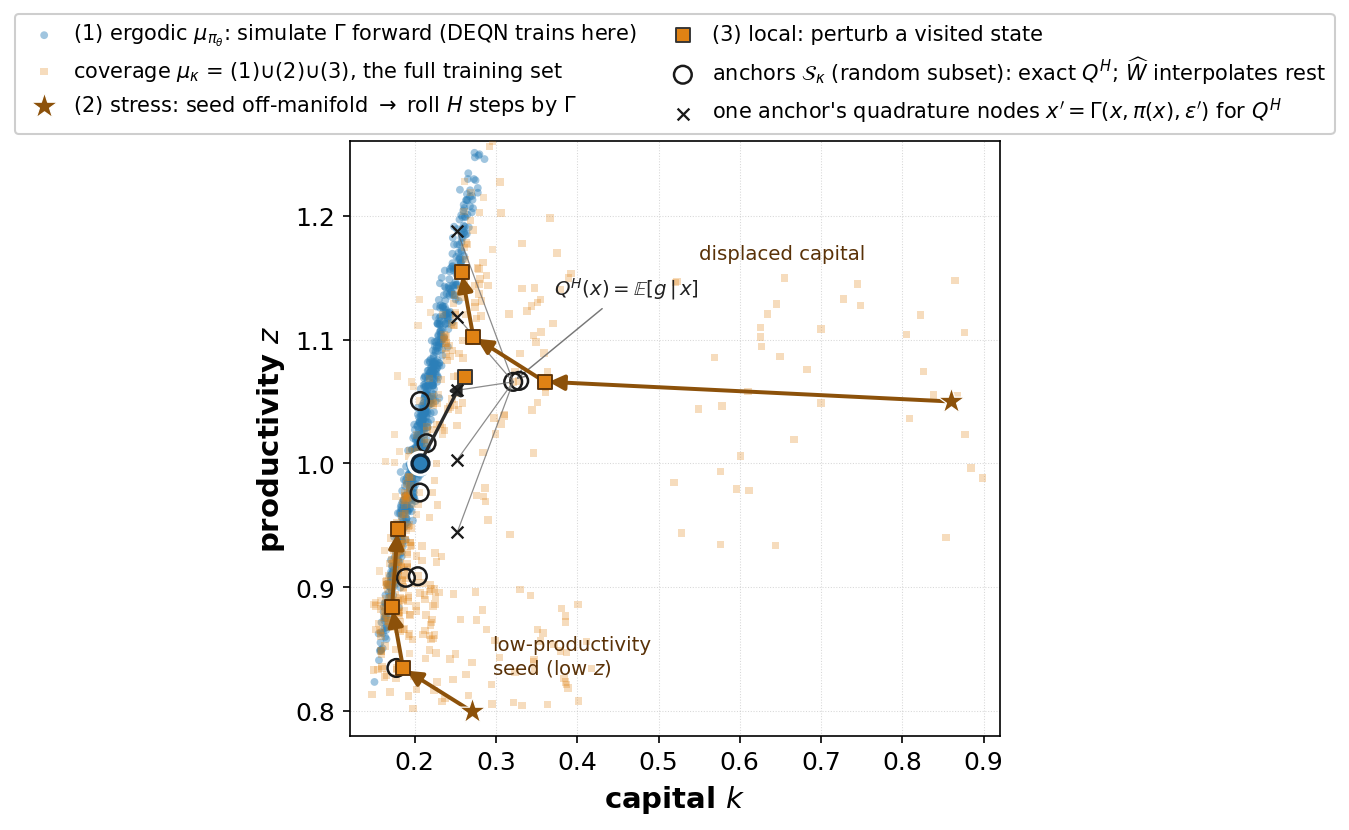
\includegraphics[width=\linewidth,height=0.52\textheight,keepaspectratio]{figures/ewm_bm_coverage_2d.png}\\[2pt]
{\footnotesize Coverage in $(K,z)$: the ergodic path plus stressed and counterfactual states, each from the exact law of motion. Schaab \& Scheidegger (2026).}
\column{0.46\textwidth}
\sloppy
The economics is tested in \emphc{rare, stressed and counterfactual} regions, exactly where pathwise training is weakest.
\vspace{0.5em}
\begin{itemize}\setlength\itemsep{8pt}
  \item In our experiments on \emphc{rare-disaster} models, the standard solver fails to find a verified solution across essentially every seed.
  \item With coverage, EWM solves in most runs and \emphc{audits} the error on the disaster region.
\end{itemize}
\vspace{0.6em}
{\footnotesize\itshape Not a new equilibrium concept, but a stronger certificate for the same one.}
\end{columns}
\end{frame}

% --- HPC ---
\begin{frame}{Data Parallelism for DEQNs}
\begin{center}
{\itshape ``To pull a bigger wagon, add more oxen rather than grow a gigantic ox.''}\\[1pt]
{\footnotesize a folk aphorism of parallel computing, usually attributed to Seymour Cray}
\end{center}
\begin{columns}[T]
\column{0.55\textwidth}
\begin{center}
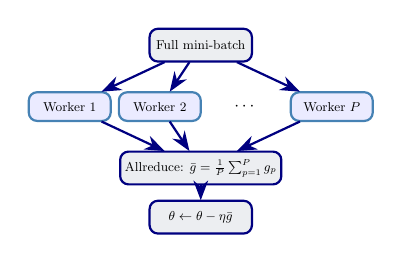
\begin{tikzpicture}[scale=0.52, transform shape,
    mlstep/.style={rectangle, draw=uzhblue, thick, fill=uzhgreylight,
        minimum width=2.5cm, minimum height=0.8cm, font=\small,
        rounded corners=3pt},
    worker/.style={rectangle, draw=softblue, thick, fill=blue!8,
        minimum width=2.0cm, minimum height=0.7cm, font=\small,
        rounded corners=3pt},
    arr/.style={-{Stealth[length=2.5mm]}, thick, uzhblue}
]
    \node[mlstep] (data) at (0,0) {Full mini-batch};
    \node[worker] (w1) at (-3.2,-1.5) {Worker 1};
    \node[worker] (w2) at (-1.0,-1.5) {Worker 2};
    \node[font=\large] (dots) at (1.1,-1.5) {$\cdots$};
    \node[worker] (wP) at (3.2,-1.5) {Worker $P$};

    \node[mlstep] (grad) at (0,-3.0) {Allreduce: $\bar{g} = \frac{1}{P}\sum_{p=1}^P g_p$};
    \node[mlstep] (upd) at (0,-4.2) {$\param \leftarrow \param - \eta \bar{g}$};

    \draw[arr] (data) -- (w1);
    \draw[arr] (data) -- (w2);
    \draw[arr] (data) -- (wP);

    \draw[arr] (w1) -- (grad);
    \draw[arr] (w2) -- (grad);
    \draw[arr] (wP) -- (grad);

    \draw[arr] (grad) -- (upd);
\end{tikzpicture}
\end{center}

\column{0.43\textwidth}
\textbf{Idea:} split the mini-batch across \emphc{multiple workers}. Each computes a local gradient on its slice, and an \emphc{allreduce} averages them before the update.

\vspace{0.4em}
\begin{itemize}\itemsep3pt\footnotesize
    \item Implemented with Horovod or MPI.
    \setlength{\itemsep}{2pt}
    \item Communication costs $\mathcal{O}(|\param|)$ per step, \emphc{independent of the data size}: the network is exchanged, not the batch.
    \item Synchronous data parallelism is close to linear for moderate worker counts; large clusters become communication-limited.
\end{itemize}
\end{columns}
\end{frame}

% --- Summary ---
\begin{frame}{Summary: What to Take Away}
\begin{columns}[T]
\column{0.52\textwidth}
\textbf{The method:}
\begin{enumerate}\itemsep4pt
    \item DEQNs replace \emphc{labels} with equations, \emphc{grids} with a network, and \emphc{time iteration} with SGD on simulated paths.
    \item Enforce what you can \emph{exactly} in the architecture; take the expectation \emph{inside} the residual, and only then square it.
    \item Validate against a benchmark; diagnose with Euler errors, never the loss curve.
\end{enumerate}

\column{0.46\textwidth}
\textbf{The practice:}
\begin{enumerate}\setcounter{enumi}{3}\itemsep4pt
    \item \emphc{Loss-scale imbalance} is the most common silent failure: normalize and rebalance.
    \item \emphc{Architecture is a numerical choice}: search it, budget it, report it.
    \item A low residual can still be a \emphc{lazy}, self-confirming policy: anchor it, audit off-path.
\end{enumerate}
\end{columns}

\vspace{0.35cm}
\begin{center}
{\footnotesize \textbf{The one-sentence version.} Solving an economic model becomes \emphc{training a neural network}, and then all the engineering that makes that training reliable becomes part of the numerical method.}
\end{center}
\end{frame}

% --- Hands-on preview ---
\begin{frame}{Deep Equilibrium Nets, Part II: 11:00 -- 12:30}
\textbf{You will build and train DEQNs yourself, starting from Brock--Mirman:}

\vspace{0.4em}
\begin{enumerate}\itemsep4pt
    \item \textbf{Deterministic Brock--Mirman}: exogenous uniform sampling of states; compare the trained policy against the closed form $s^\star = \alpha\beta$, and reproduce the validation figure from Part III. \hfill{\footnotesize\texttt{02\_01}}
    \item \textbf{Stochastic Brock--Mirman} ($\varrho > 0$, $\sigma_z > 0$): \emphc{simulation-based sampling} on the ergodic set, with Gauss--Hermite quadrature for $\Et{\cdot}$, including the node rescaling. \hfill{\footnotesize\texttt{02\_02}}
    \item \textbf{Extensions}: endogenous labor with a non-negativity constraint, which introduces a \emph{Karush--Kuhn--Tucker} multiplier $\nu_t \ge 0$ and a second loss component. \hfill{\footnotesize\texttt{02\_03}, \texttt{02\_04}}
\end{enumerate}

\vspace{0.4em}
{\footnotesize Then the two pathologies of Parts IV and V, on the same code: loss kernels (\texttt{02\_05}), architecture search (\texttt{02\_06}, \texttt{02\_07}), and loss balancing (\texttt{02\_08}).}

\vspace{0.5em}
\begin{center}
{\footnotesize \textbf{Materials:}~\href{https://github.com/sischei/summer-school-AI-for-economics-and-finance-2026}{course GitHub repository}~~$\cdot$~~\textbf{Platform:}~\href{https://nuvolos.cloud}{nuvolos.cloud} (no local setup required)}
\end{center}
\end{frame}

% --- KKT and Fischer-Burmeister ---
\begin{frame}{Exercise 3 in One Slide: KKT Without a Kink}
\textbf{The problem.} Complementary slackness bundles three conditions at once,
\[
\nu \ge 0, \qquad g \ge 0, \qquad \nu\,g = 0,
\]
and inequalities are awkward inside a smooth loss.

\vspace{0.4em}
\textbf{The trick.} The \emph{Fischer--Burmeister} function (Fischer, 1992) packages all three into one residual:
\[
\varphi_{\mathrm{FB}}(a,b) = a + b - \sqrt{a^2 + b^2},
\qquad
\varphi_{\mathrm{FB}}(a,b) = 0 \iff a, b \ge 0,\ a\,b = 0 .
\]

\begin{columns}[T]
\column{0.52\textwidth}
\begin{block}{Why the equivalence holds}
\footnotesize
For $a, b \ge 0$, $a+b=\sqrt{a^2+b^2}$ if and only if $(a+b)^2 = a^2+b^2$, that is $2ab = 0$. The function is differentiable everywhere except at the origin, and autodiff handles it directly.
\end{block}

\column{0.46\textwidth}
\begin{exampleblock}{Where Part IV comes back}
\footnotesize
The exercise loss adds a squared \emph{Euler} residual to a squared \emph{Fischer--Burmeister} residual. The two live at different scales, which makes it a textbook case for the \emphc{loss balancing} of Part IV.
\end{exampleblock}
\end{columns}
\end{frame}

% --- The book / materials ---
\begin{frame}{Want More Details? The Full Book}
\begin{columns}[c]
\column{0.40\textwidth}
\begin{center}
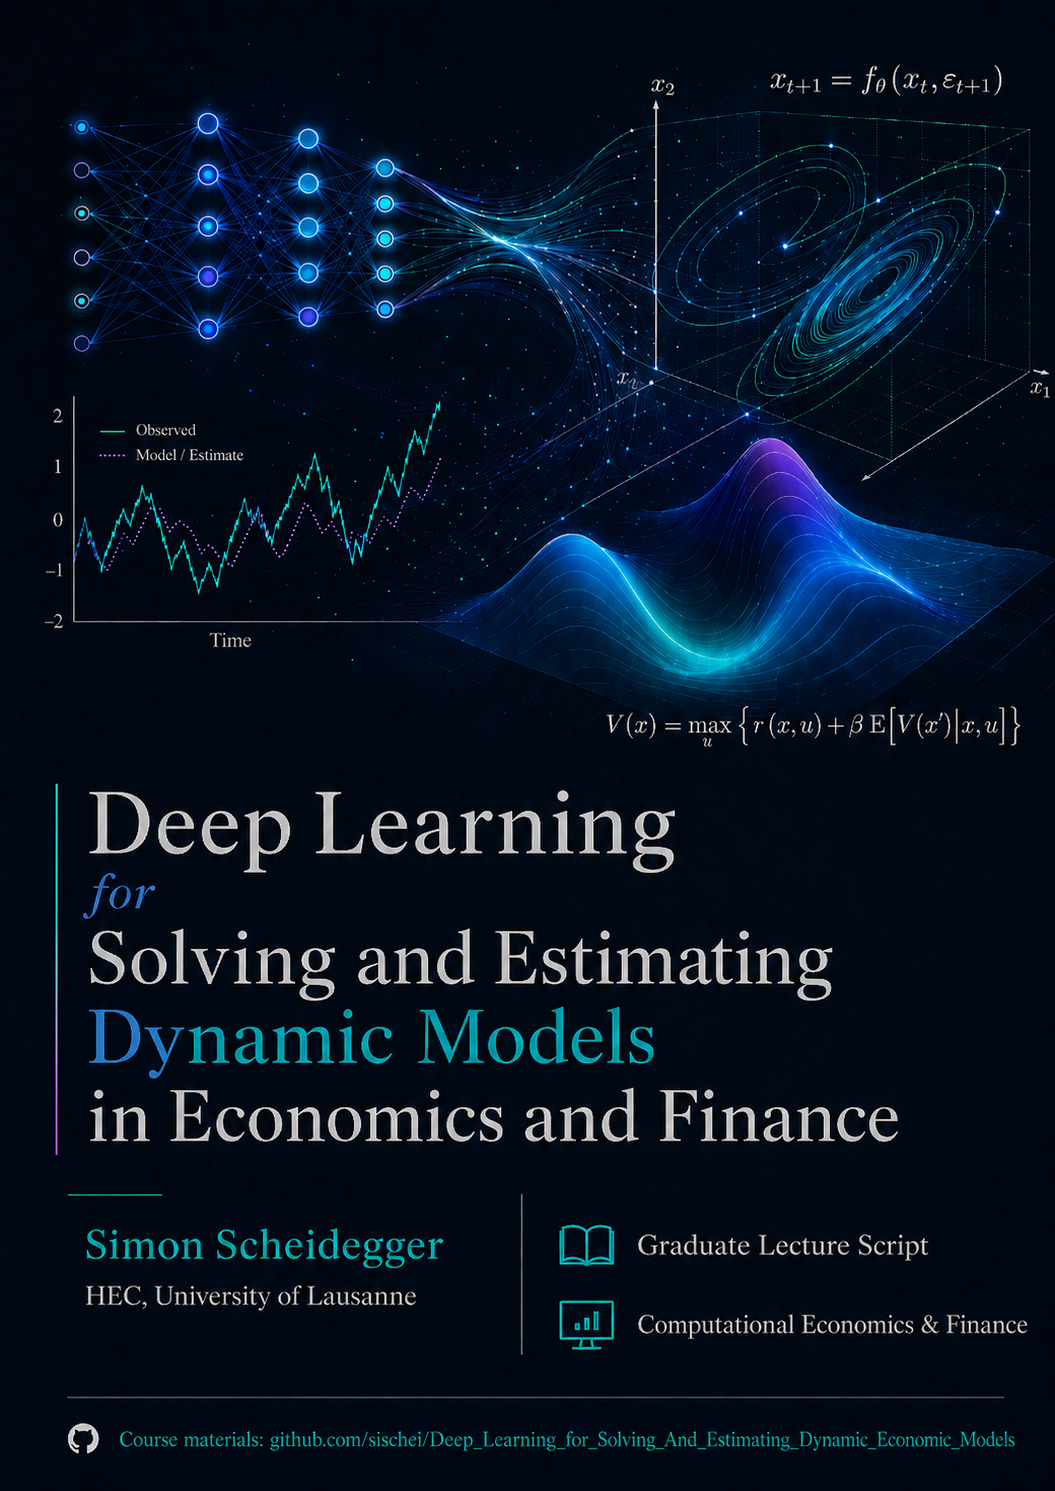
\includegraphics[height=0.70\textheight,keepaspectratio]{figures/book_hero.png}
\end{center}

\column{0.56\textwidth}
\textbf{\emphc{Deep Learning for Solving and Estimating Dynamic Models in Economics and Finance}}\\[6pt]

A book and graduate lecture script that develops these methods in full.\\[6pt]

\begin{itemize}\itemsep3pt
    \item \textbf{18 lectures}, from foundations to research-level applications.
    \item \emphc{Everything is in code}: each lecture ships with runnable notebooks.
    \item Covers what this lecture could only sketch: heterogeneous agents, occasionally binding constraints, estimation, and uncertainty quantification.
\end{itemize}

\vspace{8pt}
{\small Freely available: \href{https://github.com/sischei/Deep_Learning_for_Solving_And_Estimating_Dynamic_Economic_Models}{the book repository on GitHub}}
\end{columns}
\end{frame}

% --- Questions ---
\begin{frame}{}
\begin{columns}[c]
\column{0.45\textwidth}
\begin{center}
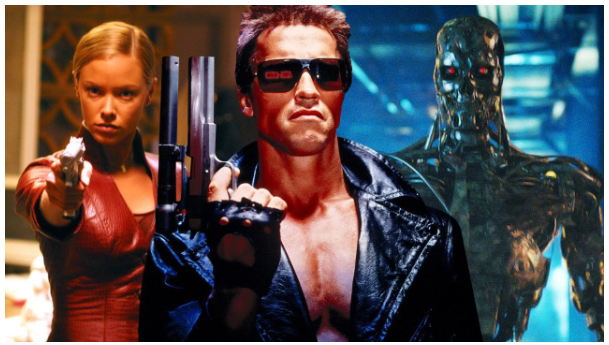
\includegraphics[width=0.85\textwidth]{figures/quest.png}
\end{center}

\column{0.50\textwidth}
\begin{center}
{\Huge \textcolor{uzhblue}{\textbf{Questions?}}}

\vspace{0.8cm}
{\large Simon Scheidegger}\\[4pt]
{\small HEC, University of Lausanne}\\[4pt]
\url{https://sischei.github.io}

\vspace{0.6cm}
{\small Next up: 11:00 -- 12:30, Deep Equilibrium Nets (part II)}\\[6pt]
{\small Materials:}\\[3pt]
{\footnotesize\href{https://github.com/sischei/summer-school-AI-for-economics-and-finance-2026}{github.com/sischei/summer-school-AI-for-economics-and-finance-2026}}\\[4pt]
{\footnotesize Platform: \href{https://nuvolos.cloud}{nuvolos.cloud}}
\end{center}
\end{columns}
\end{frame}

% ============================================================================
% APPENDIX (backup slides, shown only if time permits / on request)
% ============================================================================

\appendix

\begin{frame}{}
\begin{center}
{\Huge \textcolor{uzhblue}{Backup slides}}
\end{center}
\end{frame}

% --- GradNorm ---
\begin{frame}{GradNorm: Balance the Gradients, Not the Losses}
\begin{columns}[T]
\column{0.54\textwidth}
\textbf{Idea} (Chen et al., 2018): adjust $\omega_k$ so that the \emph{gradient norms} are balanced,
\[
    \bigl\|\nabla_{\bm{W}}\, \omega_k \, \mathcal{L}_k\bigr\|_2 \approx \bar{G} \cdot \kappa_k^{(m)} ,
\]
by descending on the auxiliary loss
\[
    \mathcal{L}_{\mathrm{grad}} = \sum_{k=1}^{M} \Bigl| \bigl\| \nabla_{\bm{W}}\, \omega_k \mathcal{L}_k \bigr\|_2 - \bar{G} \cdot \kappa_k^{(m)} \Bigr| ,
\]
with the target $\bar G \cdot \kappa_k^{(m)}$ treated as a \emphc{constant} when differentiating. The weights are learnable, $\omega_k \gets \omega_k - \eta_\omega \nabla_{\omega_k} \mathcal{L}_{\mathrm{grad}}$, then renormalized to $\sum_k \omega_k = M$.

\column{0.44\textwidth}
where
\begin{itemize}\itemsep2pt\footnotesize
    \item $\bm{W}$ is a \emphc{chosen subset of shared weights}, typically the last shared layer, which is what makes the method affordable;
    \item $\bar{G}$ is the average gradient norm over components;
    \item $\kappa_k^{(m)} = (\tilde{\mathcal{L}}_k^{(m)} / \bar{\tilde{\mathcal{L}}}^{(m)})^{\alpha_{\mathrm{gn}}}$ is the relative inverse training rate, with $\tilde{\mathcal{L}}_k^{(m)} = \mathcal{L}_k^{(m)} / \mathcal{L}_k^{(0)}$ and $\alpha_{\mathrm{gn}} \approx 1.5$.
\end{itemize}

\vspace{0.3cm}
{\footnotesize \textbf{Pros:} principled, and it addresses gradient competition directly.\\[3pt]
\textbf{Cons:} needs per-component gradients, so it is more expensive to run and more intricate to implement.}
\end{columns}
\end{frame}

% --- Bayesian optimization ---
\begin{frame}{Bayesian Optimization}
\begin{columns}[T]
\column{0.55\textwidth}
\textbf{Idea:} build a \emph{surrogate} from configuration to loss, and use it to pick the next trial.

\vspace{0.2cm}
\begin{enumerate}\itemsep2pt
    \item Fit a Gaussian process to the observed trials
    \item Compute an \emphc{acquisition function}, such as Expected Improvement
    \item Evaluate the best configuration, update, repeat
\end{enumerate}

\vspace{0.25cm}
{\footnotesize \textbf{Advantage:} \emphc{sample-efficient}: it exploits structure in the response surface.}

\column{0.42\textwidth}
\begin{block}{Expected Improvement}
\footnotesize
\[
    \text{EI}(\state) = \E{\max(f^* - f(\state), 0)}
\]
with $f^*$ the best observed value: it balances \emph{exploration} against \emph{exploitation}.
\end{block}

\vspace{0.3cm}
{\footnotesize \textbf{Cons:} inherently sequential, so harder to parallelize; the surrogate fit costs $\mathcal{O}(n^3)$ in the number of trials and degrades in high dimensions.}
\end{columns}
\end{frame}

% --- Method comparison ---
\begin{frame}{Search Strategies Compared}
\begin{center}
\renewcommand{\arraystretch}{1.3}
\begin{tabular}{@{}lccc@{}}
\toprule
\textbf{Property} & \textbf{Random} & \textbf{Bayesian} & \textbf{Hyperband} \\
\midrule
Trials to a given quality & Baseline & \emphc{Fewest} & Few \\
Cost per trial & Full training & Full training $+$ surrogate & \emphc{Early stopping} \\
Parallelization & Fully parallel & Sequential & Mostly parallel \\
\bottomrule
\end{tabular}
\end{center}

\vspace{0.4cm}
\begin{itemize}\itemsep3pt
    \item Comparing raw cost in the budget $n$ is meaningless, since $n$ is chosen. The meaningful axis is how many trials a method needs to reach a given quality.
    \item Grid search is omitted: it is dominated by random search on every axis here.
    \item Hyperband samples configurations at random, so it handles interactions exactly as well as random search. What it adds is early stopping, not a better proposal.
\end{itemize}

\vspace{0.25cm}
{\footnotesize Production tooling wraps all of these: Optuna, Ray Tune, KerasTuner, Ax.}
\end{frame}

\end{document}
